%%%%%%%%%%%%%%%%%%%%%%%%%%%%%%%%%%%%%%%%%
% Masters/Doctoral Thesis 
% LaTeX Template
% Version 2.5 (27/8/17)
%
% This template was downloaded from:
% http://www.LaTeXTemplates.com
%
% Version 2.x major modifications by:
% Vel (vel@latextemplates.com)
%
% This template is based on a template by:
% Steve Gunn (http://users.ecs.soton.ac.uk/srg/softwaretools/document/templates/)
% Sunil Patel (http://www.sunilpatel.co.uk/thesis-template/)
%
% Template license:
% CC BY-NC-SA 3.0 (http://creativecommons.org/licenses/by-nc-sa/3.0/)
%
%%%%%%%%%%%%%%%%%%%%%%%%%%%%%%%%%%%%%%%%%

%----------------------------------------------------------------------------------------
%	PACKAGES AND OTHER DOCUMENT CONFIGURATIONS
%----------------------------------------------------------------------------------------

\documentclass[
11pt, % The default document font size, options: 10pt, 11pt, 12pt
%oneside, % Two side (alternating margins) for binding by default, uncomment to switch to one side
english, % ngerman for German
singlespacing, % Single line spacing, alternatives: onehalfspacing or doublespacing
%draft, % Uncomment to enable draft mode (no pictures, no links, overfull hboxes indicated)
%nolistspacing, % If the document is onehalfspacing or doublespacing, uncomment this to set spacing in lists to single
%liststotoc, % Uncomment to add the list of figures/tables/etc to the table of contents
%toctotoc, % Uncomment to add the main table of contents to the table of contents
%parskip, % Uncomment to add space between paragraphs
%nohyperref, % Uncomment to not load the hyperref package
headsepline, % Uncomment to get a line under the header
%chapterinoneline, % Uncomment to place the chapter title next to the number on one line
%consistentlayout, % Uncomment to change the layout of the declaration, abstract and acknowledgements pages to match the default layout
]{MastersDoctoralThesis} % The class file specifying the document structure

\usepackage[utf8]{inputenc} % Required for inputting international characters
\usepackage[T1]{fontenc} % Output font encoding for international characters

\usepackage{mathpazo} % Use the Palatino font by default

%\usepackage[authordate,bibencoding=auto,strict,backend=biber,natbib]{biblatex-chicago}
\usepackage[backend=bibtex,style=authoryear,natbib=true]{biblatex} % Use the bibtex backend with the authoryear citation style (which resembles APA)

\addbibresource{references.bib} % The filename of the bibliography

\usepackage[autostyle=true]{csquotes} % Required to generate language-dependent quotes in the bibliography

\usepackage[inline]{enumitem}

\usepackage{mathtools, cases}

\usepackage{amsmath,amssymb}

\usepackage{optidef} % For writing optimisation problems

\usepackage{algorithm}
\usepackage[noend]{algpseudocode}

\usepackage{graphicx}

\usepackage{hyperref}

\usepackage{placeins}

%----------------------------------------------------------------------------------------
%	MARGIN SETTINGS
%----------------------------------------------------------------------------------------

\geometry{
	paper=a4paper, % Change to letterpaper for US letter
	inner=2.5cm, % Inner margin
	outer=3.8cm, % Outer margin
	bindingoffset=.5cm, % Binding offset
	top=1.5cm, % Top margin
	bottom=1.5cm, % Bottom margin
	%showframe, % Uncomment to show how the type block is set on the page
}

%----------------------------------------------------------------------------------------
%	THESIS INFORMATION
%----------------------------------------------------------------------------------------

\thesistitle{Using metaheuristics to solve the Agile road mapping problem} % Your thesis title, this is used in the title and abstract, print it elsewhere with \ttitle
\supervisor{Rune Møller \textsc{Jensen}} % Your supervisor's name, this is used in the title page, print it elsewhere with \supname
\examiner{} % Your examiner's name, this is not currently used anywhere in the template, print it elsewhere with \examname
\degree{MSc Software Development and Technology (Advanced Computing)} % Your degree name, this is used in the title page and abstract, print it elsewhere with \degreename
\author{Thomas \textsc{Roberts}} % Your name, this is used in the title page and abstract, print it elsewhere with \authorname
\addresses{} % Your address, this is not currently used anywhere in the template, print it elsewhere with \addressname

\subject{} % Your subject area, this is not currently used anywhere in the template, print it elsewhere with \subjectname
\keywords{Agile, Optimisation, Meta heuristics} % Keywords for your thesis, this is not currently used anywhere in the template, print it elsewhere with \keywordnames
\university{\href{https://www.itu.dk/}{IT University of Copenhagen}} % Your university's name and URL, this is used in the title page and abstract, print it elsewhere with \univname
\department{\href{https://computerscience.wikit.itu.dk/}{Computer Science Department}} % Your department's name and URL, this is used in the title page and abstract, print it elsewhere with \deptname
%\group{\href{https://ml.itu.dk/}{Machine Learning Research Group}} % Your research group's name and URL, this is used in the title page, print it elsewhere with \groupname
\group{}
%\faculty{\href{https://ml.itu.dk/}{Machine Learning Research Group}} % Your faculty's name and URL, this is used in the title page and abstract, print it elsewhere with \facname
\faculty{}

\AtBeginDocument{
\hypersetup{pdftitle=\ttitle} % Set the PDF's title to your title
\hypersetup{pdfauthor=\authorname} % Set the PDF's author to your name
\hypersetup{pdfkeywords=\keywordnames} % Set the PDF's keywords to your keywords
}

\begin{document}

\frontmatter % Use roman page numbering style (i, ii, iii, iv...) for the pre-content pages

\pagestyle{plain} % Default to the plain heading style until the thesis style is called for the body content

%----------------------------------------------------------------------------------------
%	TITLE PAGE
%----------------------------------------------------------------------------------------

\begin{titlepage}
\begin{center}

\vspace*{.06\textheight}
{\scshape\LARGE \univname\par}\vspace{1.5cm} % University name
\textsc{\Large Masters Thesis}\\[0.5cm] % Thesis type

\HRule \\[0.4cm] % Horizontal line
{\huge \bfseries \ttitle\par}\vspace{0.4cm} % Thesis title
\HRule \\[1.5cm] % Horizontal line
 
\begin{minipage}[t]{0.4\textwidth}
\begin{flushleft} \large
\emph{Author:}\\
\href{https://www.linkedin.com/in/thomas-roberts-5ba514114/}{\authorname} % Author name - remove the \href bracket to remove the link
\end{flushleft}
\end{minipage}
\begin{minipage}[t]{0.4\textwidth}
\begin{flushright} \large
\emph{Supervisor:} \\
\href{http://www.itu.dk/people/rmj/pmwiki/}{\supname} % Supervisor name - remove the \href bracket to remove the link  
\end{flushright}
\end{minipage}\\[3cm]
 
\vfill

\large \textit{A thesis submitted in fulfillment of the requirements\\ for the degree of \degreename}\\[0.3cm] % University requirement text
\textit{in the}\\[0.4cm]
\deptname\\[2cm] % Research group name and department name
 
\vfill

{\large \today}\\[4cm] % Date
%\includegraphics{Logo} % University/department logo - uncomment to place it
 
\vfill
\end{center}
\end{titlepage}

%----------------------------------------------------------------------------------------
%	DECLARATION PAGE
%----------------------------------------------------------------------------------------

\begin{declaration}
\addchaptertocentry{\authorshipname} % Add the declaration to the table of contents
\noindent I, \authorname, declare that this thesis titled, \enquote{\ttitle} and the work presented in it are my own. I confirm that:

\begin{itemize} 
\item This work was done wholly or mainly while in candidature for a research degree at this University.
\item Where any part of this thesis has previously been submitted for a degree or any other qualification at this University or any other institution, this has been clearly stated.
\item Where I have consulted the published work of others, this is always clearly attributed.
\item Where I have quoted from the work of others, the source is always given. With the exception of such quotations, this thesis is entirely my own work.
\item I have acknowledged all main sources of help.
\item Where the thesis is based on work done by myself jointly with others, I have made clear exactly what was done by others and what I have contributed myself.\\
\end{itemize}
 
\noindent Signed:\\
\rule[0.5em]{25em}{0.5pt} % This prints a line for the signature
 
\noindent Date:\\
\rule[0.5em]{25em}{0.5pt} % This prints a line to write the date
\end{declaration}

\cleardoublepage

%----------------------------------------------------------------------------------------
%	ABSTRACT PAGE
%----------------------------------------------------------------------------------------

\begin{abstract}
\addchaptertocentry{\abstractname} % Add the abstract to the table of contents
Agile methodologies split a project into short sprints where a small set of tasks are worked on. An agile team must carefully create a sprint plan that is realistic and delivers the maximum value to the customer. While this short term planning enables high agility, a longer-term road map is also useful to communicate the current state of the project to stakeholders. This planning activity can be viewed as a new take on the classic scheduling problem and in this thesis, the agile road mapping problem is formulated as an optimisation problem that assigns user stories to sprints. A solution to this problem aims to maximise the business value delivered by the road map without violating any development constraints such as overloading a sprint or placing a story before its dependencies. The problem is given an integer programming formulation and solved optimally using the IBM ILOG CPLEX Optimiser. It is then given a local search formulation and is solved using a combination of iterated local search, random restarts, simulated annealing, and tabu search metaheuristics to find approximate solutions that are close to optimal. The results of this approximate method are compared to results of the complete method, and it is shown that metaheuristics can produce good solutions in far less time than using complete algorithms.
\end{abstract}

%----------------------------------------------------------------------------------------
%	ACKNOWLEDGEMENTS
%----------------------------------------------------------------------------------------

%\begin{acknowledgements}
% \addchaptertocentry{\acknowledgementname} % Add the acknowledgements to the table of contents
% The acknowledgments and the people to thank go here, don't forget to include your project advisor\ldots
% \end{acknowledgements}

%----------------------------------------------------------------------------------------
%	LIST OF CONTENTS/FIGURES/TABLES PAGES
%----------------------------------------------------------------------------------------

\tableofcontents % Prints the main table of contents

%----------------------------------------------------------------------------------------
%	THESIS CONTENT - CHAPTERS
%----------------------------------------------------------------------------------------

\mainmatter % Begin numeric (1,2,3...) page numbering

\pagestyle{thesis} % Return the page headers back to the "thesis" style

% Include the chapters of the thesis as separate files from the Chapters folder
% Uncomment the lines as you write the chapters

%https://student.unsw.edu.au/thesis-structure

% Chapter Template

\chapter{Introduction} % Main chapter title

\label{ChapterIntroduction}

A key part of the Agile software development process is to create a sprint plan. An agile team combines their expected availability with their estimations of how large, complex and valuable their tasks are so that they can decide on which tasks will be delivered in the next sprint. The goal of this planning activity is to create a plan that delivers the most value to the customer within an iteration. While this might sound simple, even small projects can have many tasks to take into consideration and mismanaging this planning has the potential to create many operational risks. For example, taking on too many tasks increases the risk of non-delivery and can make the team seem inconsistent and unreliable. It also inevitably overloads the development team which may affect their job satisfaction. Mismanaging the business value delivered by a plan creates the risk that the team is viewed as not delivering useful software.

While an agile development team will intentionally keep the plan as short-term as possible (typically just one sprint), a longer-term plan known as a \emph{road map} can be useful for stakeholders to have an overview of the current state of the project. However, creating a road map comes with the important caveat that it can change frequently and dramatically after every sprint. Most commercial agile project management tools provide ways to create a product backlog and track the progress made on user stories using Kanban boards and burn-down charts. To create a sprint plan, one can simply sort stories by business value from largest to smallest. More advanced tools can produce Gantt charts that map out a sequence of tasks according to the dependencies between them, but these generally only try to produce feasible plans. However, the aim of sprint planning is not just to produce a feasible plan but one that maximises the amount of value delivered to the customer as early as possible.

Creating a road map can be modelled as an optimisation problem where a solution is a set of user stories assigned to sprints, the objective is to maximise the business value delivered by the road map, and constraints are used to represent development constraints such as dependencies between tasks and overloading a sprint with too much work. We refer to this problem as the Agile Sprint Planning Problem (ASPP). Complete methods have been used to find optimal solutions to the ASPP [\citet{golfarelli2012sprint}, \citet{golfarelli2013multi}]. However, it has been shown that as the size and complexity of the problem grows, the time taken to find the optimal solution grows exponentially. Results show that it can take tens of minutes to solve instances of the problem that are not uncommon in practice. Local search techniques are often used to find solutions to difficult optimisation problems that are 'good enough' by sacrificing the guarantee of optimality to gain an often substantial increase in speed.

\section{Contribution}

This thesis aims to answer the question: \emph{Can metaheuristics provide a better trade-off between computation time and solution quality for the ASPP than complete methods based on mathematical programming?} Therefore, this thesis contributes a model to the ASPP that is a set of user stories, sprints, and development constraints, and implements a metaheuristic that can find good solutions in a reasonable amount of time. In addition, it contributes a way to exploit characteristics specific to the ASPP to generate valuable solutions in the search.

This work does not contribute a user-friendly, graphical tool that will allow an agile team to create and maintain their product backlog and produce nicely-formatted sprint plans. It will focus on writing code that uses local search techniques, running the code on test data sets, and comparing the results with an implementation that uses a complete algorithm.

\section{Summary of Results}

Combining large neighbourhood search with random restarts, simulated annealing and tabu search can find solutions that are within 1\% or 2\% of the optimal in less time than using complete methods. It can be seen that when the size of the problem gets very large, the gap in value between the optimal and approximate begins to grow due to the exponential number of possible solutions. However, the number of iterations given to the approximation search is arbitrary and can be increased to a suitable amount that suits very large problems. This should make it possible to get within 1\% or 2\% of the optimal in large problems while still taking far less time than a complete algorithm. As the difficulty of problems increases, the large neighbourhood search also starts to have more difficulty but still stays within an acceptable solution quality while using less time than the complete algorithm.
% Chapter Template

\chapter{Background}\label{ChapterBackground}

This chapter gives an overview of the two important themes of this thesis: agile software development and optimisation problems. It will establish the vocabulary used throughout the rest of the paper and outline the concepts about these two topics that will give some context to the implementation and results of the work.

\section{Agile Software Development}

When writing software became less of an academic exercise and more of a commercial one, there were few frameworks available for how to manage this process. \citet{benington1983production} is cited as one of the first to suggest an approach to developing large programs inspired by the highly-structured processes used in manufacturing. It consisted of a nine stage plan that maps out the phases of a project, starting with creating a list of requirements for what the system needs to do, implementation, testing and end-user evaluation. \citet{royce1987managing} was one of the first to formalise this process and it would later become known as the Waterfall Model (notice that Royce used this model as an example of a bad way to develop software that should be avoided). Since then, many frameworks have been proposed as an alternative to waterfall that try to deliver software products on time, within budget, but most importantly, that meets the customer's expectations.

Agile software development is one such approach that has been widely adopted by development teams. Agile is the term for a collection of frameworks based on the values described in the Manifesto for Agile Software Development (\citet{beck2001manifesto}). Agile methodologies focus not only on how to organise and manage the technical work required to deliver a product, but also how to foster cohesion and collaboration both within the development team and in the organisation. Broadly, Agile methodologies aim to increase the quality of software deliveries by putting great emphasis on building and maintaining a well-functioning team that is able to deliver the functionality that the customer values the most. Empirical studies such as \citet{dybaa2008empirical} have shown that depending on the size and maturity of the development team (and the company), it can sometimes be difficult to adopt the process. However once it is adopted, it is generally seen as a positive step in managing the software development process. In particular, the human and social factors that the principles foster can create a team that is more relaxed and collaborative.

%give a summary of Scrum and the development cycle (use diagrams)

A central part of Agile is the idea of working in \emph{sprints} -- short periods of time where the development team works on tasks (known as \emph{user stories}) that deliver the most value to the customer at that moment in time. A sprint typically lasts 1 or 2 weeks but can be much shorter. Working to these very short time horizons instead of long project cycles means that if the customer's priorities change during a project, unforeseen problems occur, or entirely new requirements are added, the agile development team is able to shift focus after every sprint to accommodate this. The main roles in an agile team are the \emph{Product Owner}, the \emph{Development Team}, and the \emph{Scrum Master}.

The Product Owner may either be the customer themselves or a representative for a group of customers. They are responsible for digesting the sometimes conflicting needs of the customers and maintaining a \emph{Product Backlog} that acts as a wish list of functionality that the customers want in the product. Any item in the backlog has a chance (but not a certainty) of being implemented, and anything not in the backlog will not be implemented. Every item is given a \emph{business value} which is a relative value of importance, and the Product Owner is responsible for ensuring that the most important tasks are given top priority. They are also responsible for writing user stories that the Development Team can understand so that it is easy for them to implement and test. A clear 'Definition of Done' is essential so that the Product Owner and Development Team can agree when a user story has been delivered successfully.

The Development Team is responsible for carrying out the technical work to deliver working software. They are empowered to estimate how much effort it will take to implement each task in the Product Backlog. There has been much debate and advice about how to effectively estimate the effort of user stories \citep{cohn2004user} and the measure used in this thesis is \emph{story points}. Every agile team is free to define their own scale of story points but typically they are not equivalent to elapsed time. Instead, they indicate a combination of how difficult, uncertain, and large a task is. The team can use techniques such as Planning Poker \citep{cohn_planning_poker} to make realistic estimates that everyone agrees on. Together with the Product Owner, the Development Team may also add more user stories to the backlog, for example, if a user story is dependent on some other work to be finished before it can be started on. If a user story is judged to be too large to fit into one sprint, they can work with the Product Owner to redefine the scope of the Definition of Done and break it down into multiple smaller stories that can each be delivered within a sprint. The Development Team is also responsible for communicating their planned vacation and allocation during a sprint so that the team can plan its work.

The Scrum Master is responsible for encouraging all members of the team to work in line with the principles of the Agile Manifesto and generally try to ensure that the Development Team runs efficiently and is able to deliver what the Product Owner is asking for. They work to remove any obstacles or problems blocking the Development Team from working on the tasks they have committed to. Before a sprint starts, the team holds a sprint planning meeting where they decide on which user stories will be taken in to the coming sprint. When planning the upcoming sprint, the plan should strike a good balance between delivering high-value user stories and not overloading the Development Team. The Product Owner refines the business value estimations, the Development Team refines the story point estimations, and the Scrum Master facilitates both parties to agree on a realistic and valuable sprint plan.

\section{Combinatorial Optimisation Problems}

Combinatorial Optimisation (CO) is an area of computer science where a problem is modelled in a way that a solution can be expressed as a set of assignments of values to variables. An objective function can then take a solution as an input and return a value that indicates how good the solution is. The goal is to search the set of all possible solutions to find the optimal set of assignments that maximises or minimises the objective function (depending on what is desirable for a particular problem). Notable examples of CO problems are the Travelling Salesman Problem (TSP), the Quadratic Assignment Problem (QAP), and the Resource-Constrained Project Scheduling Problem (RCPSP). Because many real-world problems can be modelled as a CO problem, there has been much research into how to solve them. Two broad classes of approaches have emerged: complete algorithms and approximation algorithms.

\subsection{Complete Algorithms}

The set of all possible solutions to a CO problem is typically finite, so a complete algorithm that can exhaustively search every possible solution is guaranteed to find the optimal one. However, CO problems that are NP-hard \citep{garey1979computers} may take an exponentially-increasing time to solve which is impractical in most cases. The Branch and Bound algorithm \citep{land1960automatic} is the most widely-used tool for solving large-scale NP-hard combinatorial optimisation problems \citep{clausen1999branch}. It represents the solution space as a rooted tree where the root node represents a solution where none of the variables have been assigned, a node in the tree represents a partial solution, and a leaf represents a complete solution. As the algorithm traverses the tree, it maintains an upper bound on the cost function over all of the solutions it has explored so far. If a new solution has a cost above the upper bound, the branch is 'cut' because it is impossible to find a lower-cost solution in the rest of the branch. This can dramatically reduce the number of solutions that are explored while still guaranteeing to find the optimal solution. The basic algorithm starts with a pessimistic upper bound of $\infty$ but this bound is tightened as the search progresses. However in the worst case, the bound does not get close to the optimal cost so few cuts are made and the search degenerates to an exhaustive search.

\section{Approximation Algorithms}
Many real applications do not necessarily require the optimal solution to a problem and a solution that is close to optimal is sufficient. By relaxing the requirement of finding the optimal solution, approximation algorithms that converge towards the optimal but may not reach it can find a very good solution in much less time than a complete algorithm.

Constructive algorithms start with an empty or partial solution and try to make assignments until a good solution is found. These can run very fast but often give poor results compared to local search algorithms \citep{blum2003metaheuristics}. Local search algorithms start with a complete solution and try to modify some of its assignments to improve the value of the solution. Making small changes to a solution to create new but similar solutions is known as generating its \emph{neighbourhood}. A local search algorithm explores a solution's neighbourhood by generating its neighbours, comparing their values, and selecting the best neighbour to accept as the new 'current' solution. Ideally, this process can be repeated and the search follows a path of increasingly-valuable solutions until it reaches the global optimum. Local search has the additional benefit that it does not need to maintain a search tree and only one solution needs to be stored in memory, making it very memory-efficient.

As described in \citet{ahuja2002survey}, a neighbourhood search algorithm can be defined as: (1) a neighbourhood graph where a node represents a feasible solution and a directed arc $(S,T)$ indicates that $T$ is in the neighbourhood of $S$, (2) a method for searching the neighbourhood graph at each iteration, (3) a method for deciding which is the next node that the search will choose. In general, the larger the neighbourhood, the better. The local search is able to 'look' further away from its current solution and reduce its chance of becoming stuck in a small area of the solution space. However, some neighbourhoods may be very large and generating, evaluating and comparing lots of neighbours may itself take a long time and increase the overall time of the local search.

\section{Metaheuristics}

Metaheuristics are high-level strategies that are not related to a specific problem and can try to guide a local search through the solution space. Well-known metaheuristics include Hill Climbing, Random Restarts, Simulated Annealing, Tabu Search, Genetic Algorithms, Evolutionary Algorithms, and Constraint-based Local Search. Any of these techniques can be used alone or in combination with other metaheuristics to help avoid the common pitfalls of local search.

\subsection{Hill Climbing}

Steepest-descent hill-climbing search is perhaps the simplest strategy whereby the search moves through the graph of solutions by comparing all of the neighbours in its neighbourhood and accepting the highest-value neighbour. This strategy usually performs poorly as it can easily become stuck in local optima and miss the global optimum. There are several other variants of hill climbing such as stochastic hill climbing which assigns a probability of being accepted to each neighbour that is proportional to the 'steepness' of the move - i.e. how good or bad it is. It then randomly selects a neighbour according to these probabilities so that good moves have a high probability of being selected and weaker moves have a smaller (but feasible) chance of being selected. Stochastic hill climbing may converge more slowly than steepest-descent but it often yields better results. In first-choice hill climbing, rather than generating and evaluating the full neighbourhood, it randomly generates a neighbour until it finds one that improves its current solution. This can be a useful strategy with problems that have a very large neighbourhood. Random restart hill climbing performs several hill-climbing searches starting from different, random starting solutions in the hope that even if each search gets stuck in a local optimum, enough of the solution space has been explored that one of the local optima is close to the global optimum.

\subsection{Simulated Annealing}

The main issue with hill climbing search is that it moves greedily, only accepting a neighbour if it improves upon the current solution. Simulated Annealing \citep{kirkpatrick1983optimization} is a method inspired by annealing in metals where the substance is first melted to allow its atoms to flow freely, and the temperature is slowly lowered until it freezes. The substance spends relatively little time near its melting point and more time close to its freezing point. By cooling it in this way, its atoms are able to move around and find a low-energy state compared to quickly freezing it and inducing defects because the atoms solidified in a sub-optimal arrangement. This process has been adapted to combinatorial optimisation problems where a temperature is cooled during the search according to a cooling schedule. When the temperature is high, the probability of accepting a 'bad' move is high and the probability reduces as the temperature is cooled. This means that the tolerance for moving from a good solution to a worse solution is high to begin with (diversification) but over time, this tolerance reduces and the search focuses on improving the current solution (intensification). In other words, the search starts off more like a random walk of the solution space and transforms into a steepest-descent hill climbing.

\subsection{Tabu Search}

When traversing the solution graph, it is possible that the search will repeatedly visit the same set of solutions. When it enters this kind of cycle, the search stalls and it gets stuck in a local area of the graph. This can happen both when only accepting improving moves or using more complex strategies to accept non-improving moves. Tabu search \citep{glover1989tabu} tries to reduce this problem by using a form of short-term memory to remember recent moves and prevent them from being made again for a given amount of time. If a move is attempted while it is still 'banned', the search must find another move that is not banned. This encourages the search to visit unexplored areas of the solution space and limits getting stuck repeating the same moves. The definition of a move is important because if a move is defined too broadly, it may be encountered too often and the tabu list may stifle the search by banning common moves. Conversely, moves that are too rare will not occur often and the tabu list is redundant since the search may still get caught in a cycle. Similarly, the length of time that a move remains banned for can greatly impact the search's performance by banning too many or too few moves at once.


%quote some papers listed in the survey
%(see \citet{kolisch2001integrated} for a comprehensive survey).

%Slide 22 of local search lecture (Escaping local maxima)
% Chapter Template

\chapter{Literature Review}
\label{ChapterLiteratureReview}

This chapter reviews how other research has tackled the ASPP using either complete algorithms or approximate algorithms.

\section{Related Work}

\citet{golfarelli2012sprint} identifies that agile methods show promising results in overcoming problems in traditional software engineering projects. It explains how while many commercial tools support generic management of the agile process, they do not provide a way of developing the optimal sprint plan in a project to develop a data warehouse. The paper formalises the ASPP as a multi-knapsack problem with constraints, where sprints are the knapsacks and user stories are the items. The problem is categorised as \enquote{resource-constrained with renewable resources (i.e., manpower) available on a period-by-period basis. As in the basic PERT/CPM model, finish-start precedences with zero time lag are considered and no preemption of activities is allowed.} It is then given an integer programming formulation and solved using the IBM ILOG CPLEX Optimiser. The model covers the critical variables needed to plan a sprint such as sprint capacity (defined by the development team's velocity), user story business value, and user story points. It also uses an additional set of constants (measured on an ordinal scale) to model the risks associated with a user story, such as how 'critical' it is to the project as a whole and the 'uncertainty' of the estimations. Lastly, it models the 'affinity' of stories so that sets of related user stories can be identified. These non-critical variables are used to weight a user story's business value or story points so that risky stories, or stories whose siblings have been assigned to the same sprint, are perceived as more valuable to work on and are more likely to be assigned to a sprint plan. While the use case of this problem is in building a data warehouse, the model that was implemented is a general model of agile methodologies that can be applied to other domains. Their model was validated in two ways: effectiveness and efficiency. The effectiveness test was done by taking a real project (that had already been completed) from a development team and using the product backlog as the input to the model. The model was run and the optimal sprint plan was created, and this was compared to the actual sprint plan that the team had used. The team's plan was then compared to the generated plan to compare the amount of business value delivered in each sprint, the distribution of risk across sprints, and how dependencies and delays were handled. The overall results were positive as the leader of the team judged that the optimal sprint plan was an improvement over the team's own plan. Secondly, the efficiency of the model was tested by evaluating how long it took to solve problem instances of increasing size (in terms of number of stories) and complexity (in terms of number of dependencies). However, it is shown that as the size and complexity grows, the computation time grows exponentially due to an exponential increase in the search space. The authors note that solving instances of more than 100 stories, or instances with many dependencies, becomes too time-consuming. Therefore, this thesis will both extend the model and explore using metaheuristics to find a better trade-off between time and the quality of solutions compared to the mathematical programming approaches like the Branch and Bound algorithm used in \citet{golfarelli2012sprint}.

Even with a well organised backlog and a carefully designed sprint plan, it is common that some user stories are not delivered in the sprint that they were planned in. This inevitably has an impact on any stories that depend on it and on any lower-value stories that were planned for the next sprints but now need to be moved to make room for the higher-value spillover. Additionally, agile frameworks give the flexibility to add or remove stories at any point in a project's lifetime. Thus, the plan generated up front often needs to be adjusted. \citet{golfarelli2013multi} describes how a new sprint plan should accommodate for this spillover and allow new stories to be scheduled, but to minimise the disruption to the teams and external stakeholders, it is desirable that the new plan is close to the original one so that any committed due dates and resource allocations can be preserved as best as possible. The basic model given in \citet{golfarelli2012sprint} is extended with the idea of supporting smooth re-planning and is solved using the IBM ILOG CPLEX Optimiser. To begin with, a 'baseline' sprint plan is generated. When a new plan needs to be made, a 'minimum perturbation strategy' is used. This strategy is seen as a multi-objective optimisation problem that tries to maximise the value of the sprint plan while also maximising the similarity between the new sprint plan and the baseline sprint plan. The paper suggests that this can be done hierarchically where one objective dominates the other - that is, the sum of the business value is kept optimal while the similarity is maximised to the greatest extent possible without reducing the business value of the sprint plan. Alternatively, a simultaneous approach could use a weighted combination of the business value and the similarity to create a more complex objective function. Ultimately, the paper chooses the first approach since maximising the value of the new sprint plan always takes priority over the similarity to the baseline. \citet{golfarelli2013multi} focuses mainly on how to generate new plans based on an existing plan using Branch and Bound but it does not explore other approaches that could solve the ASPP, whereas this thesis will explore new ways of solving the ASPP. Since the concept of smooth re-planning is mainly an extension of the objective function and the model, the new solving methods explored in this thesis could be applied in both the baseline planning and the re-planning phases.

\citet{brezovcnik2018scrum} tackles the Scrum task allocation problem using an algorithm inspired by nature called Particle Swarm Optimisation (PSO) \citep{eberhart1995particle}. This algorithm is inspired by the behaviour of groups of natural organisms that work together to find desirable areas of a space. If the organisms start from different random positions, the swarm is able to cover most of the total space and find the best area. This approach has been applied to optimisation problems where a set of candidate solutions is treated as a swarm of particles and each 'particle' carries out a local search and moves around its local space trying to find a better solution. Each candidate solution is encoded as a vector representing its position in the solution space and has a velocity that dictates the direction that it moves after each iteration. The swarm maintains the highest-value position found so far and the velocity of each particle is influenced by the position of its own local optimum and by the best known positions found by other particles. During an iteration, each particle updates the velocities of the other particles relative to the value of its best local solution. Particles are therefore attracted to high value solutions and over time, all of the particles hopefully converge on the global optimum. The advantage of PSO is that it combines exploration of the solution space with intensification of local solutions. However, as with other local search methods, the parameters chosen by the user can have a great impact on the quality of the results. For example, if all particles can communicate with each other, a particle that is close to the global optimum (but has not yet encountered it) may be attracted away from it and pulled towards a very good (but sub-optimal) solution found by another particle in another area. It can therefore give better results to limit the set of particles that each one communicates with so that they are not influenced too heavily by others. PSO is one of a plethora of approximation techniques and this thesis will explore other techniques such as large neighbourhood search, simulated annealing, and tabu search to find if they can also be applied to the ASPP.

\citet{greer2004software} proposes a method called EVOLVE that is based on a genetic algorithm. It optimally assigns a set of customer requirements to 'increments' according to the prioritisation made by the Product Owner, precedence constraints, and resource constraints. It aims to provide a way to conduct continuous planning where a new solution can be generated from scratch to accommodate changing requirements. The genetic algorithm maintains a population of solutions where the set of assignments in a solution is represented by a 'chromosome' (for example, a text string). A fitness function takes a chromosome as input and returns a value that represents how good it is. The algorithm chooses two solutions as 'parents' according to their fitness scores and 'mates' them together. Parts of each parent's chromosome are randomly selected and combined to create a 'child' solution with a new chromosome. The child's chromosome is constructed so that sub-orderings in the parents' chromosomes also appear in the child so that the child has the same characteristics as its parents but combined in a new way. Finally, part of the child's chromosome is randomly mutated to introduce some variance in each generation.

In summary, existing research has focused on developing models that represent the ASPP in a realistic way so that solutions to the problem cater for the main constraints and objectives that a real development team aims for when planning their agile sprints. To solve the problem, researchers have focused on either using complete algorithms to find optimal solutions, or using nature-inspired approximation algorithms to find good solutions. This thesis will explore if other highly-popular approximation techniques such as large neighbourhood search, simulated annealing, and tabu search can give good results compared to complete methods based on mathematical programming.
\chapter{Technical Work}
\label{ChapterTechnicalWork}

This chapter describes the technical implementation of how the agile road mapping problem is modelled and solved in this thesis. It will first cover how instances of the problem are generated so that implementations can be tested and compared. It will explain how a model is implemented to solve the problem using a complete algorithm, and how a similar model was implemented that uses a local search algorithm to find good solutions.

\section{Random Data Generation}
\label{random_data_generation}

In order to evaluate solving methods, one needs a set of stories and sprints to assign them to. While there is some value in taking an example from a real development team, the interesting properties in terms of implementation and testing are an instance's size and complexity rather than its authenticity. Therefore, the first technical task was to write code that can generate test data, and it can be found here: \url{https://github.com/t92roberts/AgileLocalSearch/tree/master/AgileTestDataGeneration}

There are many parameters to choose when generating product backlogs and sets of sprints. The main parameter is the size of the problem so that one can see how the accuracy and execution time of an algorithm scales as the size grows. There are also parameters specific to stories (business value, story points, number of dependencies) and to sprints (capacity). These will decide how tightly-constrained the problem is and consequently how hard it is to solve.

The estimates given to user stories and sprints are highly subjective and in this project, they are chosen based on the approach suggested in \citet{cohn2004user}: a sprint lasts 2 weeks, 1 story point is equivalent to 1 ideal, uninterrupted day of development work, and one full-time equivalent (FTE) adds 8 story points of capacity to a sprint.

\subsection{Generating Sprints}
\subsubsection{Estimations}
A sprint is given a random capacity between a given minimum and maximum value (inclusive) according to a uniform probability distribution. In a real development team, the sprint capacity would be calculated using the number of story points they were able to deliver in the previous sprint minus the story point estimate of the team's planned leave during the sprint. If there is no data about the previous sprint (for example, if the team is new or has changed composition), the rule of thumb of 8 story points per FTE can be used. In this project, the development team is chosen arbitrarily as having 5 FTEs. The parameters given to the test data generation are therefore: minimum sprint capacity: 0, maximum sprint capacity: $5 \times 8 = 40$.

\subsection{Generating Stories}
\subsubsection{Estimations}
A story is given a random business value and a random story point estimate between the given minimum and maximum values (inclusive) according to a uniform probability distribution. User stories are typically prioritised using business values between 1 and 10 and given a story point estimation using a modified Fibonacci scale (1, 2, 3, 5, 8, 13). In XP, a mnemonic used to create effective user stories is INVEST \citep{wake_2003} where "S" stands for "Small". Small tasks make the scope clear and break large tasks down into manageable chunks that ideally fit within a sprint. If the complexity of a task is large, it may be estimated as 13 story points to indicate that it must be broken down further (to 8 story points or less) if it is to be worked on. In this thesis, story estimate values are set to: minimum business value: 1, maximum business value: 10, minimum story points: 1, maximum story points: 8.

\subsubsection{Number of Dependencies}
In a backlog of $n$ stories, each story can have between $0$ and $n-1$ dependencies. A dependency is defined as a story in the backlog that must be completed before the dependent story can begin. The "I" in XP's INVEST mnemonic stands for "Independent". Good user stories should "not overlap in concept, and we’d like to be able to schedule and implement them in any order". While this is not always possible in reality, the model used in this thesis tries to create a backlog where most stories have few dependencies (making them easy to schedule), and some have many dependencies (making them difficult to schedule). The number of dependencies that a story has is chosen according to a geometric probability distribution. This distribution is generated using the formula for a geometric sequence $a_n = a_{n-1}*r$ where element $a_n$ in the sequence is the probability that a story has $n$ dependencies. In this thesis, term $a_0 = 0.5$ and the common ratio is $0.5$. In other words, a story has a 50\% chance of having 0 dependencies, a 25\% chance of having 1 dependency, a 12.5\% chance of having 2 dependencies etc, up to the $n-1$th possible number of dependencies.

\subsubsection{Assigning Dependencies}
Once the number of dependencies a story will have has been decided, other stories need to be selected from the backlog and assigned as dependencies. Stories are chosen randomly according to a uniform probability distribution. Before a story can be added as a dependency, one first needs to check that it is a valid dependency. The stories and the dependencies between them can be seen as a directed, acyclic graph (DAG) where vertices represent stories and edges represent the dependency links. Randomly connecting stories as dependencies may create cycles in this graph which will cause a deadlock and make stories on the cyclic path impossible to assign without violating their dependency constraints. Therefore, when a story is selected from the backlog, it is added as a dependency and the full graph is traversed in depth-first order to detect if a cycle has been created. If a cycle is found, the dependency is removed and a new potential dependency is selected. This process is repeated until the required number of dependencies has been added or all of the stories in the backlog have been considered.

\subsection{Output}
Sprints and stories are represented by C++ classes (see \cref{sec:Model}) that hold the randomly-generated values. These C++ objects are flattened and output to CSV files so that they can be read in by code written to solve the problem.

\section{Static Data Model}\label{sec:Model}
Two C++ classes are used to model the static data representing the problem:

\subsection{Sprint}
\begin{enumerate}
    \item Sprint number - a unique identifier
    \item Sprint capacity - the maximum number of story points that can be assigned to the sprint
    \item Sprint bonus - acts as a multiplier to the business value of a user story. Sprints at the start of the road map are given a higher bonus so that it is more valuable to place stories as early as possible in the road map
\end{enumerate}

\subsection{Story}
\begin{enumerate}
    \item Story number - a unique identifier
    \item Business value - the value of the user story being delivered
    \item Story points - the effort it will take to be delivered
    \item List of dependencies - a list of story numbers
\end{enumerate}

\section{Integer Programming Formulation}
\label{sec:integer_prog_formulation}

Based on \citet{golfarelli2012sprint}, the optimisation model for the ASPP aims to construct a road map by assigning stories to sprints in a way that maximises the sum of the business value of the road map. It must assign stories to sprints without exceeding the capacity of any sprint, and it must respect the dependencies between stories by assigning all of a story's dependencies to earlier sprints in the road map. A new addition to this model is the concept of a sprint bonus that encourages placing stories as early as possible in the road map. This aims to minimise the total number of sprints used by giving the first sprint has the largest sprint bonus and the last sprint has the smallest bonus so that the model rewards placing stories as early as possible. A sprint's business value is multiplied by the sprint bonus to give a weighted business value. The optimisation model is formulated in the following way:

\begin{table}[h!]
\begin{center}
\begin{tabular}{rl} \label{}
    $x_{ij} = 1$    & if sprint $i$ contains story $j$, otherwise $0$.\\
\end{tabular}
\end{center}
\caption{Decision variables}
\label{tab:decision_variables}
\end{table}

\begin{table}[h!]
\begin{center}
\begin{tabular}{rl} \label{formulation:decision_variables}
    $\mathcal{S}$   & Set of $m$ sprints.\\
    $\mathcal{U}$   & Set of $n$ user stories.\\
    $c_i$           & Capacity of sprint $i$, measured in story points.\\
    $b_i$           & Bonus of sprint $i$.\\
    $v_j$           & Business value of story $j$.\\
    $p_j$           & Story points estimate of story $j$.\\
    $\mathcal{D}_j \subset \mathcal{U}$ & Set of stories that story $j$ depends on.\\
    $\mathcal{B}_j \subset \mathcal{S}$ & Set of sprints before the sprint that story $j$ has been assigned to.
\end{tabular}
\end{center}
\caption{Sets and constants}
\label{tab:parameters}
\end{table}

Optimising a road map is defined as:

\begin{alignat}{15}    
    & Max \sum_{i=1}^{m} \sum_{j=1}^{n} x_{ij} v_j b_i \label{eq:objective}
\end{alignat}
\normalsize

subject to

\begin{alignat}{15}    
    & \sum_{j=1}^{|\mathcal{U}|} x_{ij} p_j \leq c_i                \quad \quad && \forall i \in \mathcal{S}    \label{eq:constr1}\\ % sprint capacity
    & \sum_{i=1}^{|\mathcal{S}|} x_{ij} \leq 1                      \quad \quad && \forall j \in \mathcal{U}    \label{eq:constr2}\\ % duplicate story assignments
    & \sum_{i=1}^{|\mathcal{B}_j|} x_{ij} = |D_j|   \quad \quad && \forall j \in \mathcal{U}, \forall i \in \mathcal{B}_j \label{eq:constr3} % dependencies assigned
\end{alignat}
\normalsize

\section{CPLEX Implementation}
\label{sec:cplex_implementation}

IBM ILOG CPLEX Optimizers \citep{ibm_corporation_2018} is a software library that is able to solve combinatorial optimisation problems. This library provides a C++ API that exposes the data structures and functions needed to model and solve CO problems. CPLEX offers many algorithms to solve CO problems and in this thesis (and related work), the Branch and Bound algorithm is used to solve the ASPP optimally. When a problem has been solved, it can return the solution it found and information about how the search progressed. There are three things to define in order to use this library to model and solve a problem: the set of decision variables (and their domains), the set of constraints, and the objective function. The C++ code for the CPLEX implementation of the ASPP in this thesis can be found here: \url{https://github.com/t92roberts/Agile-Sprint-Planning}

\subsection{Decision Variables}
In the integer programming formulation in \cref{sec:integer_prog_formulation}, the decision to be made is whether sprint $i$ contains story $j$. Therefore, the decision variables are modelled as a 2-dimensional array of Boolean variables where $roadmap[i][j] = 1$ means that sprint $i$ contains story $j$, and $roadmap[i][j] = 0$ means that sprint $i$ does not contain story $j$. All decision variables are initially set to $0$.

\subsection{Objective Function}
\Cref{eq:objective} states that the optimal solution maximises the sum of the business value multiplied by each sprint's bonus value across all assignments of stories to sprints in the road map. The original model in \citet{golfarelli2012sprint} does not consider where stories are assigned in the sprint plan. Simply maximising the sum of a road map's business value produces the optimal solution but in cases where the constraints do not restrict the placement of a story, there was no preference for which sprint the stories were assigned to. The result was that the optimal set of stories were included somewhere in the road map but they were randomly scattered across the sprints. Instead, it is desirable to use the fewest sprints possible by filling the first sprint with stories, then the second sprint, then the third etc rather than stories being randomly distributed across the sprints. Therefore, in this thesis, a new addition to the original model is the concept of a sprint bonus. Every sprint is assigned a bonus where the first sprint has the largest bonus and the last sprint has the smallest bonus. The business value of a story is multiplied by the bonus of the sprint it is assigned to so that it is more valuable to assign a story to an earlier sprint than a later one. Therefore, the objective function is implemented as a CPLEX expression that iterates over the 2D array of decision variables and sums up $v_j \times b_i \times x_{ij}$. This expression is added to the ILOG model as a maximisation objective.

\subsection{Constraints}

Representing the problem as a 2D array means that a column represents a sprint and a row represents a story. This allows for an intuitive implementation of all of the constraints needed.

\subsubsection{Sprint Capacity}
\Cref{eq:constr1} ensures the sum of the story points of the stories does not exceed the sprint's capacity. A constraint is added to the CPLEX model for each sprint that ensures that this sum is less than or equal to the sprint's capacity.

\subsubsection{Duplicate Story Assignments}
\Cref{eq:constr2} ensures that each story is assigned to no more than 1 sprint. In agile sprint planning, it is valid (and actually quite common) that a story is not included in the plan at all, especially if the team is planning only 1 sprint. A story can therefore be assigned to 0 or 1 sprints. This is implemented by building an expression that sums up every domain variable $x_{ij}$ for each row $j$ (representing a story) in the 2D array. Since every decision variable is initially set to 0 when the CPLEX model is constructed (indicating that it is not yet part of the sprint plan) and set to 1 when it is included, this sum acts as a count of how many times each story $j$ was assigned to a sprint. A constraint is added to the model that ensures that the sum for each row must be less than or equal to 1.

\subsubsection{Story Dependencies}
\Cref{eq:constr3} ensures that all of story $j$'s dependencies have been assigned to a sprint before sprint $i$ where story $j$ has been assigned to. Thus, assigning story $j$ to sprint $i$ is feasible if every story $d \subseteq D_j$ has been assigned to a sprint before sprint $i$. For each story $d \subseteq D_j$, an expression is built that sums up the values in the preceding columns (sprints) on the same row (story) in the 2D array as story $d$. This expression acts as a count of how many times $d$ was assigned to a sprint before sprint $i$. A constraint is added to the model for every $d \subseteq D_j$ enforcing that this sum must be equal to 1. This ensures that the stories that story $j$ depends on have been assigned to a sprint before than sprint $i$.

\subsection{Warm Start} \label{subsec:warm_start}
As described in \cref{subsec:complete_algorithms}, Branch and Bound uses a bound on the solution value to make cuts in the search tree. If the algorithm is not given any starting point, the starting bound is $\infty$ for minimisation problems or $-\infty$ for maximisation problems. Instead, if a complete, feasible solution can be built greedily and quickly, it can give a better initial bound to B\&B. The motivation for this is that if a good incumbent solution is known from the beginning, it can start the search from an advanced position and allow cuts to be made sooner - ideally the initial solution is already close to optimal. This is known as a 'warm start' or an 'advanced start'. Warm starts can greatly improve the time to find the optimal solution but results can vary significantly depending on how good the initial solution is. If the solution is poor, the bound will not help the search, the computation time spent to build it will have been wasted, and the relative time may be longer in small problems than without a warm start.

CPLEX provides functionality to give the model a 'MIP start' where one can assign values to some or all of the decision variables before the search starts. An initial solution is generated using the same technique as described later in \cref{repair} and the corresponding assignments are inserted into a MIP start and added to the ILOG model.

\section{Metaheuristic Implementation}

The next task is to write the C++ code that models the same ASPP so that it can be solved using large neighbourhood search, and this can be found here: \url{https://github.com/t92roberts/AgileLocalSearch/tree/master/AgileLocalSearch}. In the integer programming formulation, it is modelled as a set of binary decision variables indicating if a sprint contains a story. The local search formulation is modelled so that each decision variable represents a user story and its domain is the set of sprints and solving the problem involves assigning a sprint number to every story.

While the goal is to assign stories to sprints, it is also a valid assignment to keep a story in the product backlog if other stories can deliver more value, if there is no sprint capacity to place it, or if its dependencies have not been delivered/planned. When the data is loaded, one extra sprint is added. This special sprint has 0 sprint bonus and infinite capacity and represents the product backlog. If a story is assigned to this sprint, it doesn't add any value to the road map but it is still a valid assignment if there is nowhere to place it in the available sprints. Therefore when the problem is being solved using metaheuristics, $m + 1$ sprints are used whereas in the integer programming formulation, there are $m$ sprints.

\subsection{Pseudo code}

\begin{algorithm}[H]
\caption{Large Neighbourhood Search}\label{metaheuristic}
\begin{algorithmic}[1]
    \Procedure{LNS}{$\mathcal{S}, \mathcal{U}$}
        \State $\textit{best solution} \gets \textit{randomAssignment}(\mathcal{U}, \mathcal{S})$
        \State $\textit{current solution} \gets \textit{best solution}$
        
        \While {$iteration < a$}
            \If {$\textit{unaccepted iterations} > a / 10$}
                \State $\textit{best solution} \gets \textit{randomAssignment}(\mathcal{U}, \mathcal{S})$
            \EndIf
            
            \State $\textit{destroyed solution} \gets \textit{destroy}(\textit{current solution})$
            \State $\textit{repaired solution} \gets \textit{repair}(\textit{destroyed solution})$
            
            \If {$\textit{accept}(\textit{repaired solution, current solution})$}
                \State $\textit{current solution} \gets \textit{repaired solution}$
                
                \If {$\textit{value}(\textit{current solution}) > \textit{value}(\textit{best solution})$}
                    \State $\textit{best solution} \gets \textit{current solution}$
                \EndIf
            \EndIf
        \EndWhile
        
        \State \Return {$\textit{best solution}$}
    \EndProcedure
\end{algorithmic}
\end{algorithm}

\Cref{metaheuristic} shows the high-level logic of the metaheuristic that has been implemented. It uses a combination of large neighbourhood search, random restarts, tabu search, and simulating annealing to search the state space and return the best solution it can find in the given time.

Line 2 constructs a solution that will be the starting 'best' solution of the search. It does this by shuffling the set of all stories so that they are in a random order and greedily assigns them to sprints (see \cref{repair}). Because the search has not started yet, Line 3 sets the current solution as the initial best one. Lines 4 - 12 are the main loop of the algorithm that carry out the search. Line 4 shows that the search will terminate after a fixed number of $a$ iterations. Lines 5 and 6 show the random restarts step where if the search does not accept a new solution for one-tenth of the total number of iterations, a new solution is randomly generated in the same way as in Line 2 and the search continues from this new starting point. Lines 7 and 8 perform the large neighbourhood steps where Line 7 partially destroys the current solution by removing some of the stories from the sprint they are assigned to create an incomplete solution (see \cref{destroy}) and Line 8 repairs the partial solution by reinserting the removed stories to create a new, complete solution (see \cref{repair}). Line 9 determines if the new solution should be accepted as the new candidate solution and replace the current one (see \cref{acceptance}). Lines 11 and 12 check if the newly-accepted solution is better than the current best one found so far during the entire search and replaces it if so.

\subsection{Destroy} \label{destroy}

Two strategies are used to destroy a solution: random and radial. These are applied alternately to allow the search to add some variety to the neighbour generation.

\subsubsection{Random Destruction}

Random destruction is the simplest approach where stories are randomly chosen from the set of all stories and removed from whichever sprint they are currently assigned to. While random destruction is a relatively crude technique, it is an effective way to encourage diversification in the search as every story has the chance of being reassigned, thereby reducing the chance of becoming stuck in local maxima. \Cref{random_destruction} outlines the steps to achieve this destruction.

\begin{algorithm}[H]
\caption{Random Destruction}\label{random_destruction}
\begin{algorithmic}[1]
    \State $r \gets \textit{number of stories to remove}$
    
    \Procedure{RandomDestroy}{$\mathcal{S}, \mathcal{U}, r$}
        \State $\mathcal{R} \gets \textit{set of removed stories}$
        \State $\mathcal{M} \gets \textit{set of moves}$
        
        \While{$|\mathcal{R}| < r \land |\mathcal{U}| > 0$}
            \State $story \gets \textit{random story} \in \mathcal{U}$
            \State $sprint \gets AssignedSprint(story) \in \mathcal{S}$
            \State $Unassign(story, sprint)$
            
            \State $\mathcal{R} \gets \mathcal{R} \cup story$
            \State $\mathcal{U} \gets \mathcal{U} \setminus story$
            \State $\mathcal{M} \gets \mathcal{M} \cup Move(story, sprint)$
        \EndWhile
        
        \State \Return{$\mathcal{S}, \mathcal{U}, \mathcal{M}$}
    \EndProcedure
\end{algorithmic}
\end{algorithm}

Lines 5 - 11 are the main loop that removes stories from their sprints. Line 5 shows that the loop repeats until the required number of stories has been removed or there are no more stories available to consider. Line 6 randomly selects a story from the solution and Line 7 gets the sprint that it is assigned to. Line 8 then unassigns the story from its sprint. Line 9 adds the story to the set of removed stories and Line 10 removes the story from the solution so that it is not considered again in this round of destruction. Line 11 creates a move that represents the opposite action of removing the story from its sprint (i.e. adding the removed story back in to the sprint it was just removed from), and the move is added to the set of moves. This move will later be checked against the tabu list and adding the reverse move ensures that the action will not be undone for a given number of iterations.

\subsubsection{Radial Destruction}

While random destruction can prove effective, the characteristics of a specific problem can be exploited to heuristically decide which assignments to remove. \citet{shaw1998using} describes that while there are many strategies to do this, a general approach is to remove \textit{related} assignments. In vehicle routing problems, Shaw suggested that related visits could be those that are geographically close to one another, on the same route, or have similar allowable visiting hours. A relatedness measure that uses one or a combination of these heuristics defines how related two visits are. This general strategy can be adapted to other problems and in the ASPP, the relatedness measure is a binary value indicating whether two stories are directly or indirectly connected in the DAG of dependencies. We refer to this as 'radial' destruction because one story is chosen as the starting point, its immediate dependencies are removed, and the removal radiates outwards through the graph in breadth-first order. \Cref{radial_destruction} shows how this is done.

\begin{algorithm}[H]
\caption{Radial Destruction}\label{radial_destruction}
\begin{algorithmic}[1]
    \State $r \gets \textit{number of stories to remove}$
    
    \Procedure{RadialDestroy}{$\mathcal{S}, \mathcal{U}, r$}
        \State $\mathcal{R} \gets \textit{set of removed stories}$
        \State $\mathcal{M} \gets \textit{set of moves}$
        
        \While{$|\mathcal{R}| < r \land |\mathcal{U}| > 0$}
            \State $story \gets \textit{random story} \in \mathcal{U}$
            \State $\mathcal{R} \gets \mathcal{R} \cup BFS(story)$
            
            \For{$\textit{removed story} \in \mathcal{R}$}
                \State $\mathcal{U} \gets \mathcal{U} \setminus \textit{removed story}$
                \State $\textit{assigned sprint} \gets AssignedSprint(\textit{removed story})$
                \State $Unassign(story, sprint)$
                \State $\mathcal{M} \gets \mathcal{M} \cup \textit{(removed story, sprint)}$
            \EndFor
        \EndWhile
        
        \State \Return{$\mathcal{S}, \mathcal{U}, \mathcal{M}$}
    \EndProcedure
\end{algorithmic}
\end{algorithm}

Lines 5 - 12 are the main loop that removes stories from their sprints. Line 5 shows that the loop repeats until the required number of stories has been removed or there are no more stories to remove. Line 6 randomly selects a story from the solution. Line 7 uses this story as the root of the sub-tree in the breadth-first search (BFS). The BFS function traverses the story's dependency graph and adds its direct and indirect dependencies to the set of removed stories. When the BFS finishes traversing the sub-tree, Lines 8 - 12 remove the assignments from the solution. Line 9 removes the story from the solution so that it is not considered again in this round of destruction. Line 10 gets the sprint that it was assigned to and Line 11 unassigns the story from this sprint. Line 12 creates a move representing the opposite action to the removal of the story from its sprint and adds it to the set of moves. This move will later be checked against and/or added to the tabu list and adding the reverse move ensures that the action will not be undone for a given number of iterations.

To implement the breadth-first search, a story is chosen at random from the set of all stories. This is treated as the root of a sub-tree in the graph of dependencies and this sub-tree is traversed in breadth-first order. As a story is visited during the traversal, it is removed from the sprint it is assigned to. The traversal continues until the required number of stories have been removed. Traversing the tree in breadth-first order ensures that the immediate dependencies of the 'root' story are removed first, and if more stories need to be removed, the dependencies of those immediate dependencies are then removed. If the full sub-tree is traversed but more stories need to be removed, a story that has not already been visited is chosen at random and the same process is repeated.

\subsubsection{Level of Destruction}

A critical parameter for destroying a solution is how much of the solution to destroy (i.e. how many assignments should be removed) per iteration. Removing only 1 assignment forces the algorithm to progress very slowly and may increase the chance of getting stuck in a small area of the solution space, especially when the acceptance criteria described in \cref{acceptance} might restrict the size of the neighbourhood even further. Conversely, removing 100\% of the assignments degenerates the search to a random walk. The level of destruction in this paper was chosen experimentally as 15\%.

An issue with removing a fixed number of stories is that it can make it difficult to reinsert stories into a new position due to the set of constraints. To illustrate this issue, if Story 2 depends on Story 1, and Story 1 has no dependencies, Story 1 can be placed in Sprint 1 and Story 2 in Sprint 2 - the dependency constraints are initially satisfied. However, if Story 1 is now removed and placed in Sprint 3 (or back into the product backlog), its own dependency constraints are satisfied but now Story 2's dependency constraints have been violated. Therefore, a decision needs to be made: either enforce that all stories connected by a dependency are removed \emph{in both directions} (i.e. recursively remove Story 1's dependencies and the stories that depend on Story 1) or allow a fixed number of stories to be removed and permit infeasible assignments. The first method ensures that every candidate solution is feasible but there is no guarantee that the global optimum can be reached through a sequence of feasible solutions. The second method means that many iterations might be 'wasted' by generating intermediate, infeasible solutions to allow the search to progress which cannot be accepted as the new best solution. In this thesis, the second option is used so that the sprint capacity constraint is enforced but the dependency constraint is relaxed. However, only feasible solutions are allowed to replace the best solution found so far.

\subsection{Repair} \label{repair}

Once a solution has been partially destroyed, it must be repaired back into a complete solution. \citet{shaw1998using} uses a branch and bound technique to find the optimal way to reinsert the removed assignments. The benefit of this approach is that the resulting repaired solution is guaranteed to improve the objective function as much as possible based on the destroyed solution. The motivation is that depending on how much of the solution has been destroyed, most of the assignments have already been made. Therefore, it is more feasible to run a 'heavyweight' algorithm like branch and bound on this much smaller subset of the solution space. However, the price of using complete algorithms like branch and bound is that even a subset of the solution space can still be quite large and it still takes time to exhaustively search it. \citet{ropke2006adaptive} chooses to use a selection of insertion heuristics including a basic greedy heuristic so that visits in the vehicle routing problem can be reinserted in a fast (but approximate) way. Similarly in this thesis, a greedy heuristic is used to repair a destroyed solution. The greedy heuristic is shown in \cref{greedy_insert}.

\begin{algorithm}[H]
\caption{Greedy Insertion}\label{greedy_insert}
\begin{algorithmic}[1]
    \State $\mathcal{I} \gets \textit{set of user stories to insert into the destroyed solution}$
    
    \Procedure{Insert Stories}{$\mathcal{I}, \emph{roadmap}$}
        \State $\mathcal{M} \gets \textit{set of moves}$
        
        \While{$|\mathcal{I}| > 0$}
            \State $\emph{story} \gets \mathcal{I}_0$
            
            \For{$\textit{sprint} \in \mathcal{S}$}
                \If {$ValidInsert(story, sprint)$}
                    \State $AssignStoryToSprint(story, sprint)$
                    \State $\mathcal{I} \gets \mathcal{I} \setminus \emph{story}$
                \EndIf
            
                \State $\mathcal{M} \gets \mathcal{M} \cup \textit{(story, sprint)}$
            \EndFor
        \EndWhile
        
        \State \Return{$roadmap, \mathcal{M}$}
    \EndProcedure
\end{algorithmic}
\end{algorithm}

For every story that was removed, the repair algorithm tries to insert it into the earliest feasible sprint to maximise the bonus received from the sprint bonus. To determine the order in which stories are reinserted, the set of removed stories are sorted according to 4 factors (with the next sorting condition used to break ties in the previous): business value, story points, number of dependencies, and number of dependees. Firstly, they are sorted by business value (largest to smallest) because intuitively, it is desirable to assign high-value stories to early sprints. Secondly, stories are sorted by story points (smallest to largest) so that it tries to fit as many stories into early sprints as possible. Next, they are sorted by the number of dependencies they have (smallest to largest) and the number of dependees (smallest to largest). The assumption here is that stories with many dependency links are difficult to assign to early sprints because many other stories must have been assigned before them. Therefore, assigning stories with fewer dependency links first may increase the chance of being able to assign highly-constrained stories in later sprints, especially when the solution has been destroyed using radial destruction. In summary, this greedy heuristic can be described as trying to reinsert the highest-value, lowest effort stories, and least-constrained stories to the earliest sprint possible.

\subsection{Acceptance Criteria} \label{acceptance}

When a new solution has been generated by destroying and repairing the current solution, the algorithm must decide whether to accept the new solution and move the search forward. The simplest approach is to only accept a new solution if it improves upon the current solution. This shortsightedness can cause the search to get stuck in a small area of the solution space and never break free to explore other areas where the globally-optimum solution might be. It is therefore desirable to allow the search to break out of a local maximum. In this thesis, two acceptance criteria are blended together to try to mitigate some of these issues: tabu search and simulated annealing.

\begin{algorithm}[H]
\caption{Acceptance criteria}\label{acceptance_criteria}
\begin{algorithmic}[1]
    \State $\textit{delta} \gets \textit{new solution value} - \textit{current solution value}$
    \State $\mathcal{M} \gets \textit{set of moves made during repair}$
    
    \If {$\textit{delta} > 0$}
        \Return {$True$}
    \EndIf
    
    \For {$move \in \mathcal{I}$}
        \If {isTabu(Move)}
            \Return {$False$}
        \EndIf
    \EndFor
    
    \If {$exp(\frac{delta}{temperature})$ < random number}
        \Return {$True$}
    \EndIf
    
    \State \Return {$\textit{False}$}
\end{algorithmic}
\end{algorithm}

\Cref{acceptance_criteria} shows the acceptance criteria used to decide if a new solution should replace the current solution and move the search forwards.

Line 1 calculates the difference in value between the new solution and the current one. If the delta is positive, it improves the search's result and Line 2 accepts it immediately.
Lines 4 - 6 check if any of the moves made during repair are in the tabu list. If so, the new solution is not accepted. Line 8 has the simulated annealing acceptance probability that compares how bad the solution is with the current temperature and accepts the new solution according to the acceptance probability. If none of the acceptance criteria accept the new solution, Line 10 rejects it.

\subsubsection{Simulated Annealing} \label{simulated_annealing}

As previously mentioned, only accepting improving solutions can lead to finding a local optimum and potentially missing the global optimum. A way to avoid this problem is to relax the requirement of only accepting improving solutions. By allowing non-improving solutions to be accepted, the search is able to move through undesirable areas of the solution space in the hope that it can arrive in a new area that has high-value solutions.

The cooling schedule is a key parameter of simulated annealing as cooling too slowly keeps the search more like a random walk that isn't able to explore local areas, and cooling too quickly doesn't allow it to break free of low-value areas. \citet{kirkpatrick1983optimization} uses a geometric cooling schedule with a cooling rate of 90\% so that temperature $T$ at time $x$ is given by $T_x = T_{x-1} \times 0.9$. The initial temperature $T_0$ is chosen so that almost every move will be accepted. Therefore, the initial temperature can have as much of an impact on performance as the cooling schedule. \citet{kirkpatrick1983optimization} suggests that the optimal starting temperature is the worst possible move between two neighbouring solutions in the entire solution space. The annealing acceptance probability tries to judge how bad a move is, and a good way to judge this is to compare it to the worst possible move. However, finding the worst move is impractical because one must enumerate all moves to find the largest delta. An estimation of the worst move can be found by generating a subset of solutions and finding the largest delta between them. \Cref{annealing_initial_temp} shows how a subset of solutions is randomly generated and the objective function value is stored in a list. The MaxDifference function shown in \Cref{max_difference} finds the smallest and largest values and returns the delta between them. This delta is used an approximation of the worst possible move and is used as the starting temperature $T_0$ in the simulated annealing implementation in this thesis (to see other approaches to this problem, \citet{ben2004computing} explores more complex heuristics for finding a good starting temperature).

\begin{algorithm}[H]
\caption{Initial temperature}\label{annealing_initial_temp}
\begin{algorithmic}[1]
    \State $\mathcal{S} \gets \textit{set of all sprints in a solution}$
    \State $\mathcal{U} \gets \textit{set of all user stories in a solution}$
    
    \Procedure{Initial Temperature}{$\mathcal{S}, \mathcal{U}$}
        \State $\mathcal{V} \gets \emph{empty set of solution values}$
        
        \For{$\textit{0} \to (|\mathcal{S}| \times |\mathcal{U}|)$}
            \State $\mathcal{V} \gets \mathcal{V} \cup value(\emph{random roadmap})$
        \EndFor
        
        \State \Return{$maxDifference(\mathcal{V})$}
    \EndProcedure
\end{algorithmic}
\end{algorithm}

\begin{algorithm}[H]
\caption{Maximum Difference}\label{max_difference}
\begin{algorithmic}[1]
    \Procedure{maxDifference}{$\mathcal{V}$}
        \State $min \gets \mathcal{V}_0$
        \State $max \gets \mathcal{V}_1$
    
        \For{$v \in \mathcal{V}$}
            \If {$v < min$}
                \State $min \gets v$
            \Else{}
                \If{$v > max$}
                    \State $max \gets v$
                \EndIf
            \EndIf
        \EndFor
        
        \State \Return{$max - min$}
    \EndProcedure
\end{algorithmic}
\end{algorithm}

\subsubsection{Tabu Search} \label{tabu}

The first task in implementing tabu search is to define what a move is for the ASPP. This can be a difficult choice to make because defining moves that are too unique can mean that there are too few 'hits' in the tabu list, making it redundant. Conversely, moves that are too common may get many hits and prevent the search from progressing. In the case of agile road map generation, destroying and repairing a solution involves removing a story from a sprint and assigning it to another sprint. When a story is being assigned to a sprint, it is desirable that it is not assigned back into the sprint it was removed from for a number of iterations. Therefore, a move is defined as inserting a story in to a sprint. When story $j$ is removed from sprint $i$ during destruction, the opposite move is added to the tabu list ($j \rightarrow i$) to prevent story $j$ from being re-inserted into sprint $i$ during the repair phase.

The second task is to decide how long a move is prohibited for (its \textit{tenure} in the tabu list). This is also a difficult choice to make because moves that are banned for too short of a time will result in too few hits in the list, and too long of a tenure may result in many hits which will stagnate the search and prevent it from progressing. Choosing a value that works for many instances of the problem a priori is hard and while the tenure chosen in this thesis is somewhat arbitrary, it uses the observation that the tenure should be a function of the difficulty of the problem. The difficulty of the problem (in terms of the number of sprints and stories) defines how many possible moves there are and consequently the possible size of a solution's neighbourhood. Intuitively, small, highly-constrained problems will have fewer possible moves while large, lightly-constrained problems will have many possible moves. Therefore, the tenure should correlate with this so that small, difficult problems have a short tenure and large, easy problems have a long tenure. The tenure in this work was chosen experimentally as $0.1 \times m \times n$.

Finally, tabu search prevents repeatedly revisiting the same moves but in some cases, getting to a new best solution can only be done by making a banned move. \citet{glover1989tabu} outlines how \textit{aspiration criteria} should be used to ensure that an improving move is always accepted, even if it uses a move that is in the tabu list since it must be a new solution. In this implementation, if a new solution is better than the current one (the delta between a new and the current solution is positive), the new solution is accepted straight away and the tabu list is not checked. If the delta is 0 or negative, all of the repair moves are checked against the tabu list in the way shown by \Cref{tabu_check}.

\begin{algorithm}[H]
\caption{Check if a move is tabu}\label{tabu_check}
\begin{algorithmic}[1]
    \Procedure{MoveIsTabu}{$move$}
        \If {$\textit{move} \in \textit{tabu list}$}
            \If {$\textit{current iteration - tabu tenure > expiration iteration}$}
                \State $\textit{removeFromTabulist(move)}$
                \State \Return {$\textit{False}$}
            \Else{}
                \State \Return {$\textit{True}$}
            \EndIf
        \Else{}
            \State \Return {$\textit{False}$}
        \EndIf
    \EndProcedure
\end{algorithmic}
\end{algorithm}
% Chapter Template

\chapter{Results}
\label{ChapterResults}

This chapter will evaluate how the local search performs compared to the complete algorithm. It will start with a simple iterated local search and show how adding metaheuristics impact the quality of the solution found and the time it takes to return the solution.

\section{Experimental Setup}
All experiments were run on a machine with an Intel Core i7-7700HQ 2.80GHz 64-bit, x64-based processor, 8 GB of DDR4 1200 MHz RAM, and running Windows 10 Home Edition.

\section{Test Data}
The sets of test data are generated using the code described in \cref{random_data_generation}. To test how the algorithms perform as the size of the problem grows, sets of $10, 20, 30, ..., 100$ stories and sprints were generated. Because the data is built randomly, there is the possibility that a data set may be highly constrained or loosely constrained purely by chance. Therefore, 3 different sets of each size are generated and the results are aggregated to control for any variance in the complexity of the data sets.

\Cref{fig:sprints} shows the capacities of the sprints, grouped by how long the road map is (the number of sprints). \Cref{fig:stories} shows how many dependencies the test data sets have, grouped by the size of the product backlog, and \cref{fig:dependencies_stories} shows how complex the backlog is in terms of how many dependencies there are between stories.

\begin{figure}[h!]
    \centering
    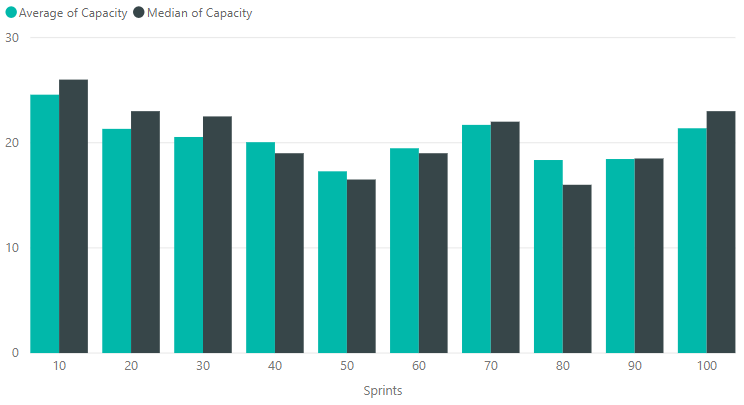
\includegraphics[width=0.8\textwidth]{Figures/TestData/sprints.png}
    \caption{Sprint capacities vs number of sprints}
    \label{fig:sprints}
\end{figure}

\begin{figure}[h!]
    \centering
    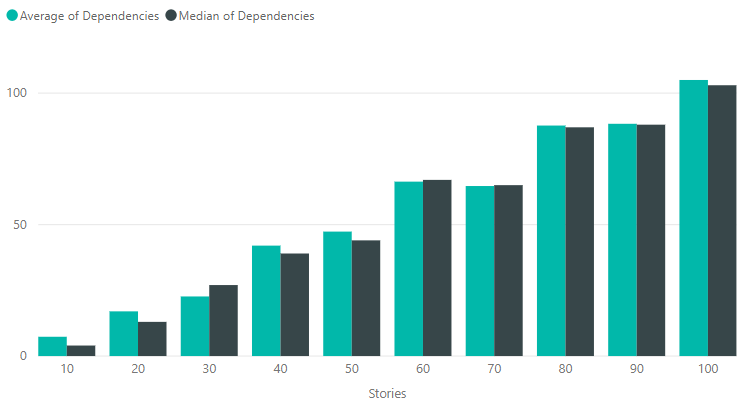
\includegraphics[width=0.8\textwidth]{Figures/TestData/stories.png}
    \caption{Number of dependencies vs number of stories}
    \label{fig:stories}
\end{figure}

\begin{figure}[h!]
    \centering
    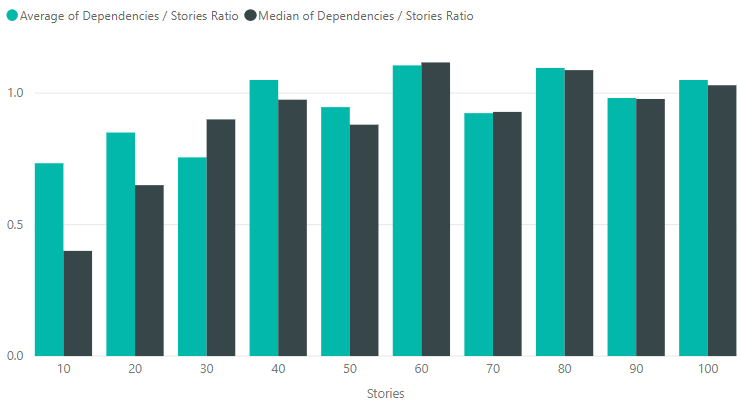
\includegraphics[width=0.8\textwidth]{Figures/TestData/dependencies_stories_ratio.png}
    \caption{Ratio between the number of dependencies and the size of the product backlog}
    \label{fig:dependencies_stories}
\end{figure}

\section{CPLEX Results}

To judge the performance of the local search implementation, the test data was first solved using CPLEX to find the optimal solution to each test problem. The optimal value and the time taken to find it could then be used as a comparison to the local search.

\subsection{Warm vs Cold Starts}

As described in \cref{subsec:warm_start}, CPLEX can use warm starts to improve its performance by giving an initial solution to the Branch and Bound algorithm. This was attempted here and \cref{fig:warm_vs_cold_starts_time} shows that the median time using warm starts was 13\% faster than cold starts. Since this is a very high-level aggregation of the results, it is also interesting to see how warm starts improved the time according to different measures such as the size or difficulty of the problem. \Cref{fig:warm_vs_cold_starts_size} shows that warm starts improved the time across most sizes of problems. \Cref{fig:warm_vs_cold_starts_stories_sprints_ratio} and \cref{fig:warm_vs_cold_starts_dependencies_stories_ratio} similarly show that warm starts matched or improved the time across most difficulties of problems. Therefore in the next section, the metaheuristics results are compared to finding the optimal solution when using warm starts.

\begin{figure}[h!]
    \centering
    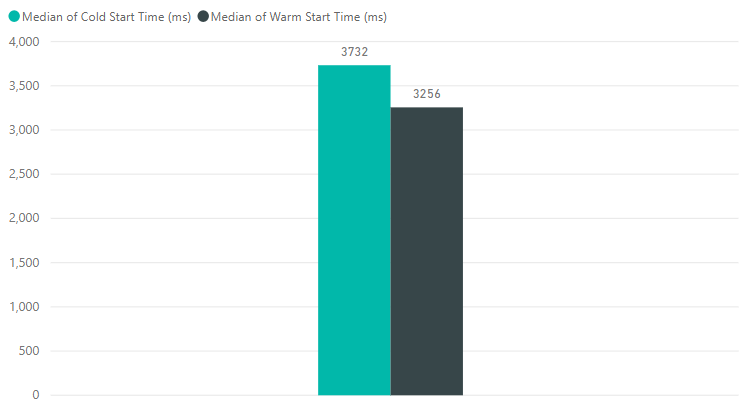
\includegraphics[width=\textwidth]{Figures/WarmVsColdStarts/warm_vs_cold_time.png}
     \caption{Median time using cold starts vs warm starts}
     \label{fig:warm_vs_cold_starts_time}
\end{figure}

\begin{figure}[h!]
    \centering
    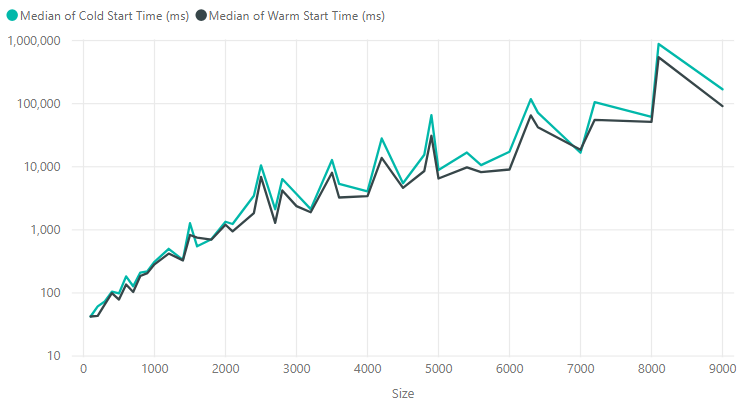
\includegraphics[width=\textwidth]{Figures/WarmVsColdStarts/warm_vs_cold_size.png}
     \caption{Median time of cold starts vs warm starts compared to the size of the problem (shown on a logarithmic scale)}
     \label{fig:warm_vs_cold_starts_size}
\end{figure}

\begin{figure}[h!]
    \centering
    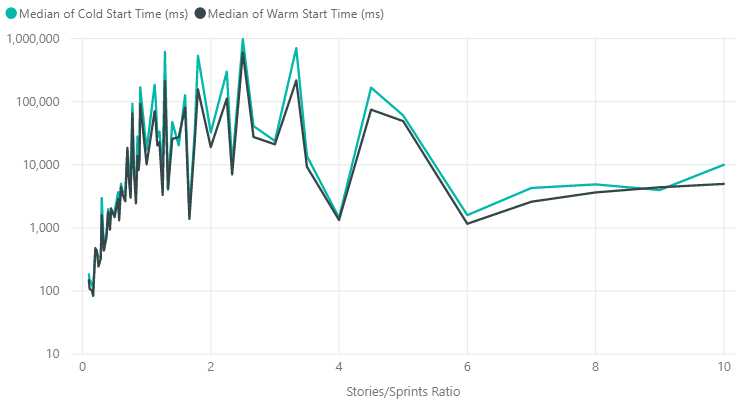
\includegraphics[width=\textwidth]{Figures/WarmVsColdStarts/warm_vs_cold_stories_sprints_ratio.png}
     \caption{Median time of cold starts vs warm starts compared to the ratio of stories to sprints (shown on a logarithmic scale)}
     \label{fig:warm_vs_cold_starts_stories_sprints_ratio}
\end{figure}

\begin{figure}[h!]
    \centering
    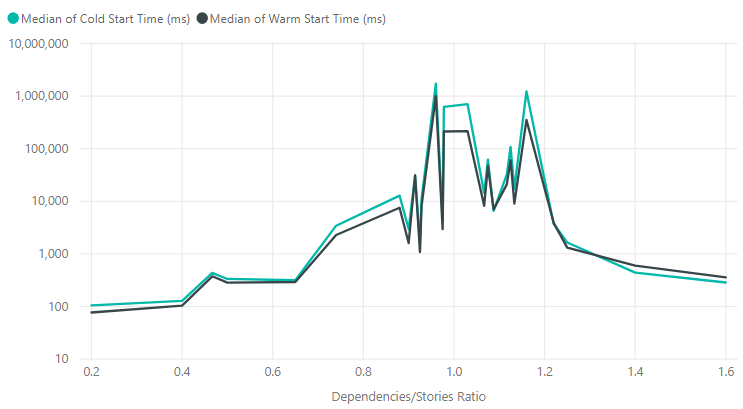
\includegraphics[width=\textwidth]{Figures/WarmVsColdStarts/warm_vs_cold_dependencies_stories_ratio.png}
     \caption{Median time of cold starts vs warm starts compared to the ratio of dependencies to stories (shown on a logarithmic scale)}
     \label{fig:warm_vs_cold_starts_dependencies_stories_ratio}
\end{figure}

\FloatBarrier

\section{Metaheuristic Results}

The metaheuristic algorithm uses randomness at many stages of the search and one execution may produce results that are different to another execution on the same data set. To control for this uncertainty, the metaheuristic algorithm was run 3 times on each test problem and the results are aggregated. To give context to the results, the value gap represents how close the solutions produced by the metaheuristic are, where 0\% means that they are equal (the metaheuristic found the optimal) and 10\% means that the metaheuristic was 10\% below the optimal value. For the time gap, 0\% means that the metaheuristic took exactly the same time as the optimal approach, +10\% means that the metaheuristic was 10\% faster than the optimal approach, and -10\% means that the metaheuristic was 10\% slower than the optimal approach.

Before diving into the comparison of adding each metaheuristic, a summary of the results is given first. The best results were found by using a combination of large neighbourhood search, random restarts and simulated annealing. Adding Tabu search gave slightly worse (but still very good) value solutions in relatively more time than the former combination. When using hill climbing, random restarts and simulated annealing, \cref{fig:value_vs_size} shows that even as the size of the problem grows, the value of solutions found is not significantly impacted and remains close to optimal.

\begin{longtable}[c]{|c|c|}
\caption{Size vs Value gap \% (best and worst highlighted)}
\label{fig:value_vs_size}\\
\hline
\textbf{Size (stories x sprints)} & \textbf{Median Value Gap \%} \\ \hline
\endfirsthead
%
\multicolumn{2}{c}%
{{\bfseries Table \thetable\ continued from previous page}} \\
\hline
\textbf{Size (stories x sprints)} & \textbf{Median Value Gap \%} \\ \hline
\endhead
%
\rowcolor[HTML]{67FD9A} 
100 & 0 \\ \hline
\rowcolor[HTML]{67FD9A} 
200 & 0 \\ \hline
300 & 0.79 \\ \hline
\rowcolor[HTML]{67FD9A} 
400 & 0 \\ \hline
500 & 0.91 \\ \hline
600 & 0.32 \\ \hline
700 & 1.35 \\ \hline
800 & 0.52 \\ \hline
900 & 0.68 \\ \hline
1000 & 1.02 \\ \hline
1200 & 0.41 \\ \hline
1400 & 0.63 \\ \hline
1500 & 0.76 \\ \hline
1600 & 0.49 \\ \hline
1800 & 1.17 \\ \hline
2000 & 0.58 \\ \hline
2100 & 0.78 \\ \hline
2400 & 0.67 \\ \hline
2500 & 0.93 \\ \hline
2700 & 0.9 \\ \hline
2800 & 0.63 \\ \hline
3000 & 1 \\ \hline
3200 & 1.38 \\ \hline
3500 & 0.76 \\ \hline
3600 & 0.91 \\ \hline
4000 & 1.22 \\ \hline
4200 & 0.73 \\ \hline
4500 & 0.63 \\ \hline
\rowcolor[HTML]{FD6864} 
4800 & 1.45 \\ \hline
4900 & 0.53 \\ \hline
5000 & 0.82 \\ \hline
5400 & 0.72 \\ \hline
5600 & 1 \\ \hline
6000 & 0.7 \\ \hline
6300 & 0.59 \\ \hline
6400 & 1.16 \\ \hline
7000 & 0.55 \\ \hline
7200 & 1.13 \\ \hline
8000 & 0.73 \\ \hline
8100 & 1.36 \\ \hline
9000 & 0.79 \\ \hline
10000 & 0.47 \\ \hline
\end{longtable}

Another measure of difficulty is how constrained the problem is. In the ASPP, this can be defined in two ways: the ratio of dependencies to stories, and the ratio of stories to sprints. \Cref{dependencies_stories_ratio_vs_value_gap} shows that the quality of solutions decreases when the ratio of dependencies to stories is close to 1, and \cref{stories_sprints_ratio_vs_value_gap} shows that the solution quality decreases when the ratio of stories to sprints is high. In both cases, this is where the problem is most constrained and the search finds it the most difficult to destroy and repair the candidate solution and may have to traverse through many infeasible solutions before it finds an improving feasible solution.

\begin{table}[h!]
\centering
\caption{Dependencies/stories ratio vs value gap \%\\(best and worst highlighted)}
\label{dependencies_stories_ratio_vs_value_gap}
\begin{tabular}{|c|c|}
\hline
\textbf{Dependencies/Stories Ratio} & \textbf{Median Value Gap \%} \\ \hline
\rowcolor[HTML]{67FD9A} 
0.2 & 0 \\ \hline
\rowcolor[HTML]{67FD9A} 
0.4 & 0 \\ \hline
0.5 & 0.15 \\ \hline
0.7 & 0.2 \\ \hline
0.9 & 0.7 \\ \hline
1 & 1.1 \\ \hline
\rowcolor[HTML]{FD6864} 
1.1 & 2 \\ \hline
1.2 & 1.05 \\ \hline
1.3 & 0.5 \\ \hline
\rowcolor[HTML]{67FD9A} 
1.4 & 0 \\ \hline
\rowcolor[HTML]{67FD9A} 
1.6 & 0 \\ \hline
\end{tabular}
\end{table}

\begin{table}[h!]
\centering
\caption{Stories/sprints ratio vs value gap \%\\(best and worst highlighted)}
\label{stories_sprints_ratio_vs_value_gap}
\begin{tabular}{|c|c|}
\hline
\textbf{Stories/Sprints Ratio} & \textbf{Median Value Gap \%} \\ \hline
\rowcolor[HTML]{67FD9A} 
0.1 & 0 \\ \hline
\rowcolor[HTML]{67FD9A} 
0.2 & 0 \\ \hline
\rowcolor[HTML]{67FD9A} 
0.3 & 0 \\ \hline
0.4 & 0.25 \\ \hline
0.5 & 0.1 \\ \hline
0.6 & 0.35 \\ \hline
0.7 & 0.3 \\ \hline
0.8 & 0.55 \\ \hline
0.9 & 0.85 \\ \hline
1 & 0.7 \\ \hline
1.1 & 1 \\ \hline
1.2 & 1.05 \\ \hline
1.3 & 1.5 \\ \hline
1.4 & 1 \\ \hline
1.5 & 1.1 \\ \hline
1.6 & 2.4 \\ \hline
1.7 & 0.9 \\ \hline
1.8 & 1.8 \\ \hline
2 & 2.1 \\ \hline
2.3 & 3.1 \\ \hline
2.5 & 1.9 \\ \hline
2.7 & 4.8 \\ \hline
3 & 3.2 \\ \hline
3.3 & 2.4 \\ \hline
3.5 & 2.6 \\ \hline
4 & 3 \\ \hline
4.5 & 6.2 \\ \hline
5 & 4.6 \\ \hline
6 & 2.4 \\ \hline
7 & 3.6 \\ \hline
8 & 5.2 \\ \hline
\rowcolor[HTML]{FD6864} 
9 & 8 \\ \hline
10 & 3.9 \\ \hline
\end{tabular}
\end{table}

\FloatBarrier

\Cref{fig:time_vs_size} shows that using the complete method usually terminated faster than the metaheuristic in small problems but the metaheuristic was usually faster in large problems. Similarly, \cref{fig:time_vs_dependencies_stories} and \cref{fig:time_vs_stories_sprints} show that as the complexity of the problems increase, the local search can find close-to-optimal solutions in a similar time in easy problems and much faster in difficult problems.

\begin{figure}[h!]
    \centering
    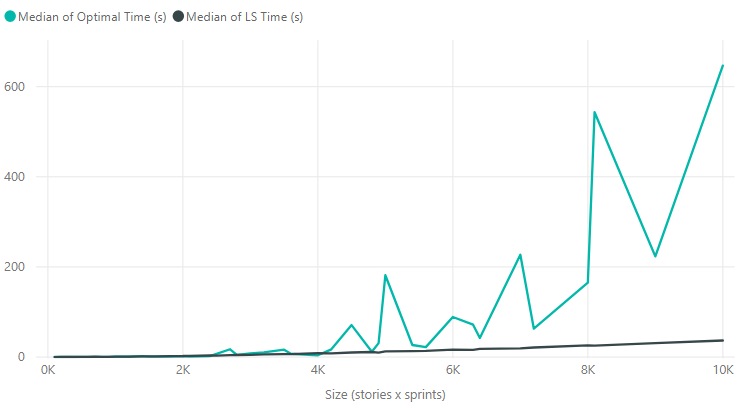
\includegraphics[width=\textwidth]{Figures/FinalResults/annealing_time_size.png}
     \caption{Size vs time - positive gap means the metaheuristic method was faster}
     \label{fig:time_vs_size}
\end{figure}

\begin{figure}[h!]
    \centering
    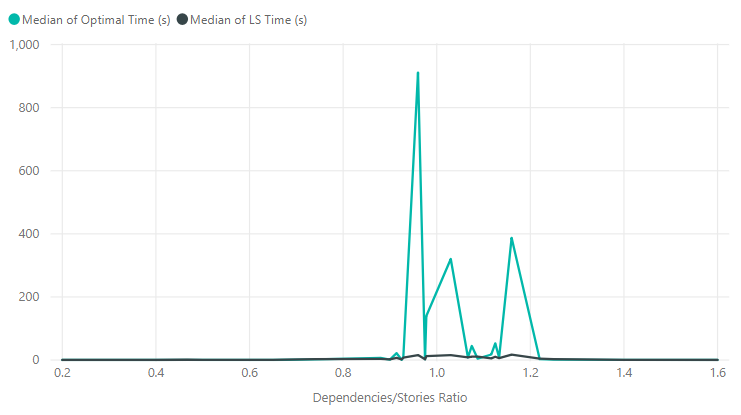
\includegraphics[width=\textwidth]{Figures/FinalResults/annealing_time_dependencies_stories.png}
     \caption{Ratio of dependencies to stories vs time - positive gap means the metaheuristic method was faster}
     \label{fig:time_vs_dependencies_stories}
\end{figure}

\begin{figure}[h!]
    \centering
    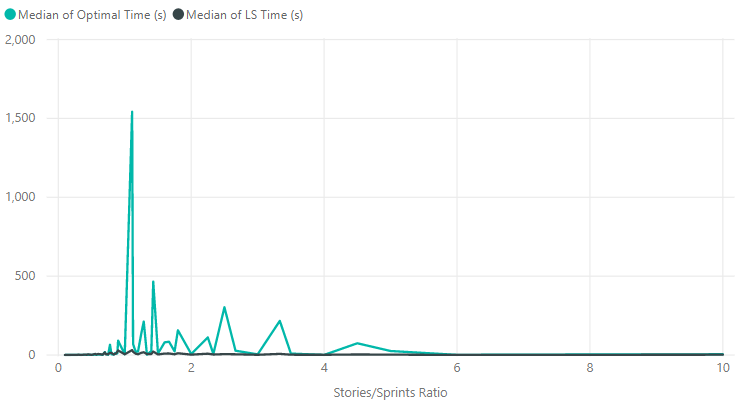
\includegraphics[width=\textwidth]{Figures/FinalResults/annealing_time_stories_sprints.png}
     \caption{Ratio of stories to sprints vs time - positive gap means the metaheuristic method was faster}
     \label{fig:time_vs_stories_sprints}
\end{figure}

\FloatBarrier

\subsection{Comparison of Metaheuristics}

To test how each metaheuristic impacts the value and time of finding approximate solutions, the metaheuristic algorithm was first run using only large neighbourhood search (LNS) where only improving candidate solutions are accepted (also known as hill climbing). Using this is a baseline, other metaheuristic strategies were cumulatively added in the following order: random restarts (restarts), simulated annealing (SA), tabu search (TS). To compare the impact of adding each metaheuristic, \Cref{fig:value_gap_perc_vs_heuristic} and \cref{fig:time_gap_perc_vs_heuristic} show the value gap and time gap (respectively) when adding each metaheuristic. It is important to note that these results are aggregated at a high level across problem instances of very different sizes and difficulties and these results are shown only to illustrate the general trend - a more detailed analysis of the results is given in \cref{subsec:result_distributions}. The results shows that even the basic hill climbing can get within 1.65\% (average) / 0.95\% (median) of the optimal value but the standard deviation is relatively high, suggesting that it gives inconsistent results. Adding random restarts closes the value gap to 1.34\% (average) / 0.71\% (median) and takes approximately the same amount of time. This is expected because hill climbing and random restarts were given the same number of iterations, but the latter was allowed to restart up to 10 times within that number of iterations if the search stagnated. Adding simulated annealing slightly improved the value gap but the time gap noticeably worsened. However, the median time gap shows that it still performed 9\% faster than the complete algorithm. Adding tabu search slightly increased the value gap and dramatically increased the time gap.

The small increase in the value gap when using tabu search could be because the search is getting stalled when the tabu list forbids accepting certain moves. Possible reasons for this could be the definition of the move or the length of the tabu tenure. On reflection, a better definition of a move could have been to have the concept of a departure sprint and a destination sprint. The tabu list would then prevent moving a story from its destination sprint back to its departure sprint whereas the definition used in this thesis was only to prevent a story being moved back to its departure sprint (i.e. it could not be moved from \emph{any} sprint back to its departure sprint while it was tabu). It could also be due to the fact that neighbours are generated stochastically and there may be cases where several successive neighbours are generated but all contain the same banned moves. As long as there is the chance that a move that was already recently found to be tabu can appear in successive neighbours (effectively a 'random choice with replacement' approach), the search may stall. On one hand, this is precisely the job of the tabu list so that the search is encouraged to explore new areas, but ultimately, preventing the search from accepting neighbours costs iterations that may have led to higher-value solutions. The worse time gap could simply be due to the additional overhead of creating moves during destruction, checking moves, and generally managing the tabu list. This overheard is low in small problems but since both the size of the tabu list and the tabu tenure are functions of the size of the problem, this overhead grows as the size of the problem grows (although it does only grow linearly). Additionally, \cref{subsec:result_distributions} will show that most 

\begin{figure}[h!]
    \centering
    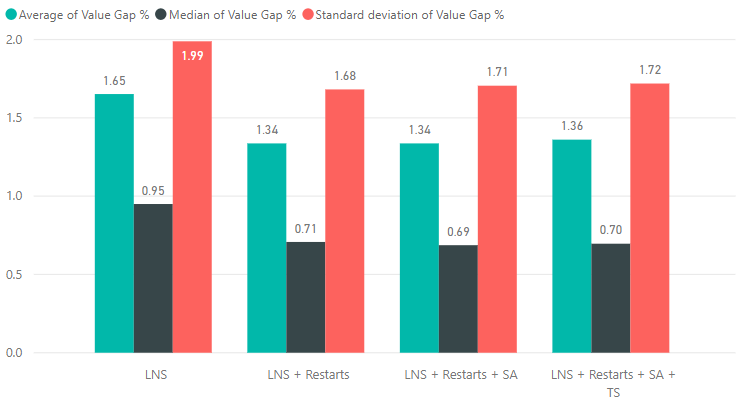
\includegraphics[width=\textwidth]{Figures/Metaheuristics/value_gap_perc_vs_heuristic.png}
    \caption{Heuristics vs Value Gap \%}
    \label{fig:value_gap_perc_vs_heuristic}
\end{figure}

\begin{figure}[h!]
    \centering
    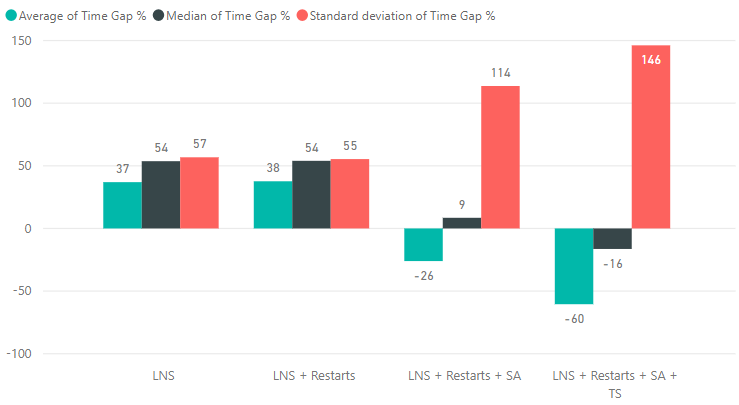
\includegraphics[width=\textwidth]{Figures/Metaheuristics/time_gap_perc_vs_heuristic.png}
    \caption{Heuristics vs Time Gap \% (positive gap means the metaheuristic method was faster)}
    \label{fig:time_gap_perc_vs_heuristic}
\end{figure}


\subsection{Result Distributions}
\label{subsec:result_distributions}

\Cref{fig:value_gap_perc_hill_climb}, \cref{fig:value_gap_perc_restarts}, \cref{fig:value_gap_perc_annealing} and \cref{fig:value_gap_perc_tabu} show the distribution of the gap between the value and time compared to the complete algorithm when adding each metaheuristic. The interesting result shown by these figures compared to the high-level aggregated results in the previous section is that most solutions were within 1\% in all combinations of metaheuristics. The basic hill climbing was able to find solutions within 0.5\% of the optimal but some were up to 15\% away from the optimal. The key improvement that adding random restarts, simulated annealing and tabu search made is to 'shift' the distribution of the value gaps to the left and the distribution of the time gaps to the right. In other words, while there are still outliers in the value and time gaps, adding the metaheuristics found better solutions in less time in most cases.

\begin{figure}[!htbp]
    \centering
    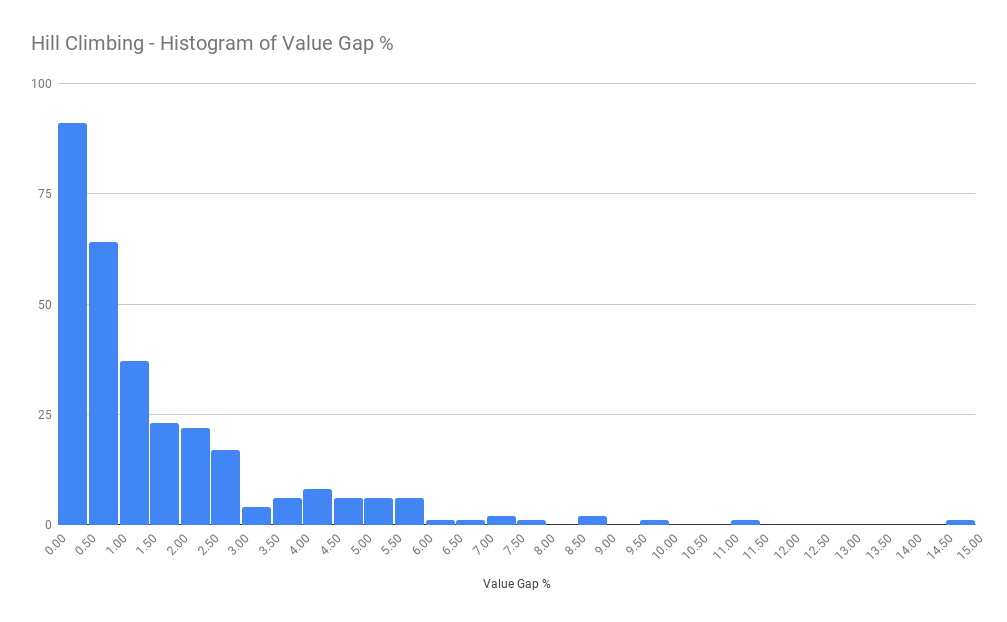
\includegraphics[width=\textwidth]{Figures/Metaheuristics/hill_climb_value_gap.png}
    \caption{LNS (Hill Climbing) Value Gap \%}
    \label{fig:value_gap_perc_hill_climb}
\end{figure}

\begin{figure}[!htbp]
    \centering
    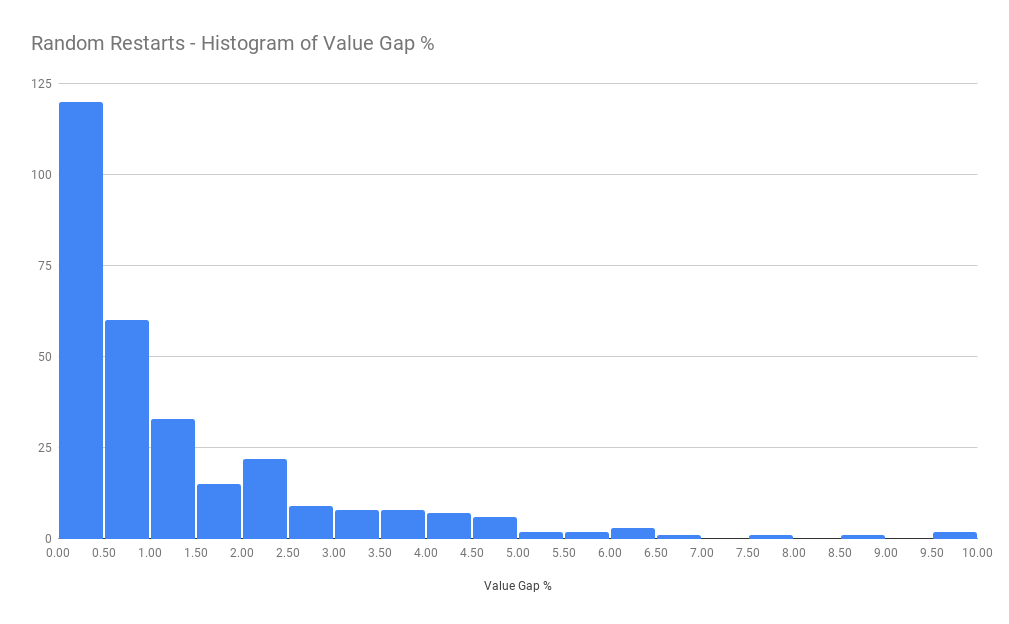
\includegraphics[width=\textwidth]{Figures/Metaheuristics/restarts_value_gap.png}
    \caption{LNS + Random Restarts Value Gap \%}
    \label{fig:value_gap_perc_restarts}
\end{figure}

\begin{figure}[!htbp]
    \centering
    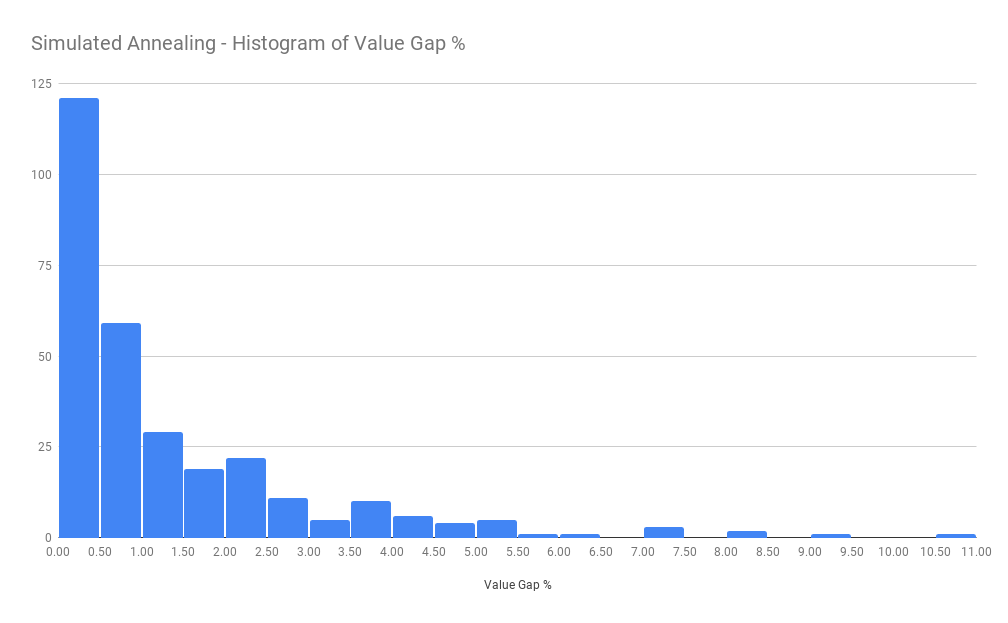
\includegraphics[width=\textwidth]{Figures/Metaheuristics/annealing_value_gap.png}
    \caption{LNS + Random Restarts + SA Value Gap \%}
    \label{fig:value_gap_perc_annealing}
\end{figure}

\begin{figure}[!htbp]
    \centering
    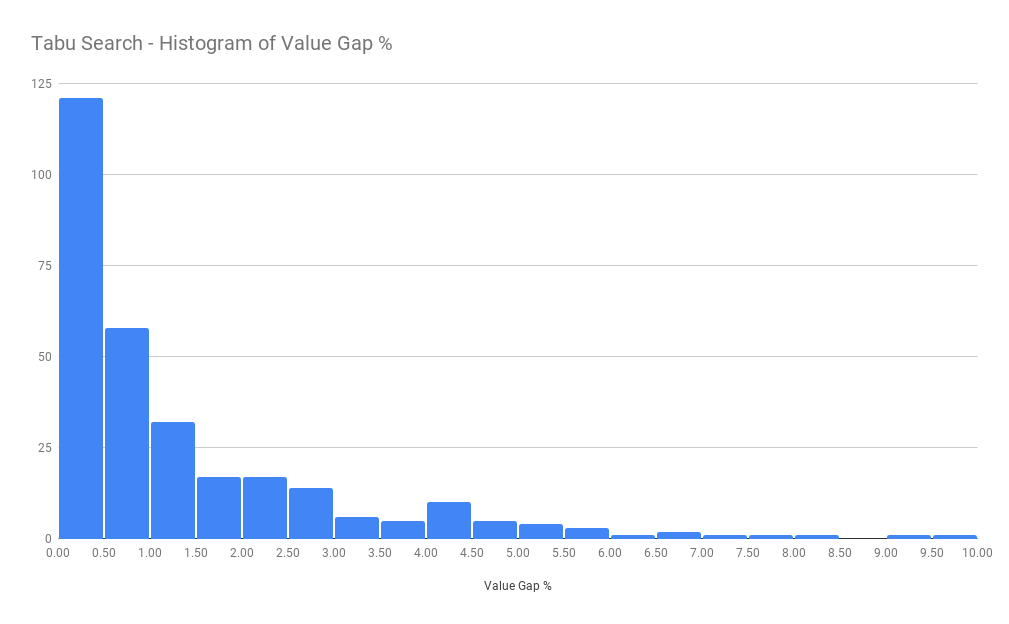
\includegraphics[width=\textwidth]{Figures/Metaheuristics/tabu_value_gap.png}
    \caption{LNS + Random Restarts + SA + TS Value Gap \%}
    \label{fig:value_gap_perc_tabu}
\end{figure}

\begin{figure}[!htbp]
    \centering
    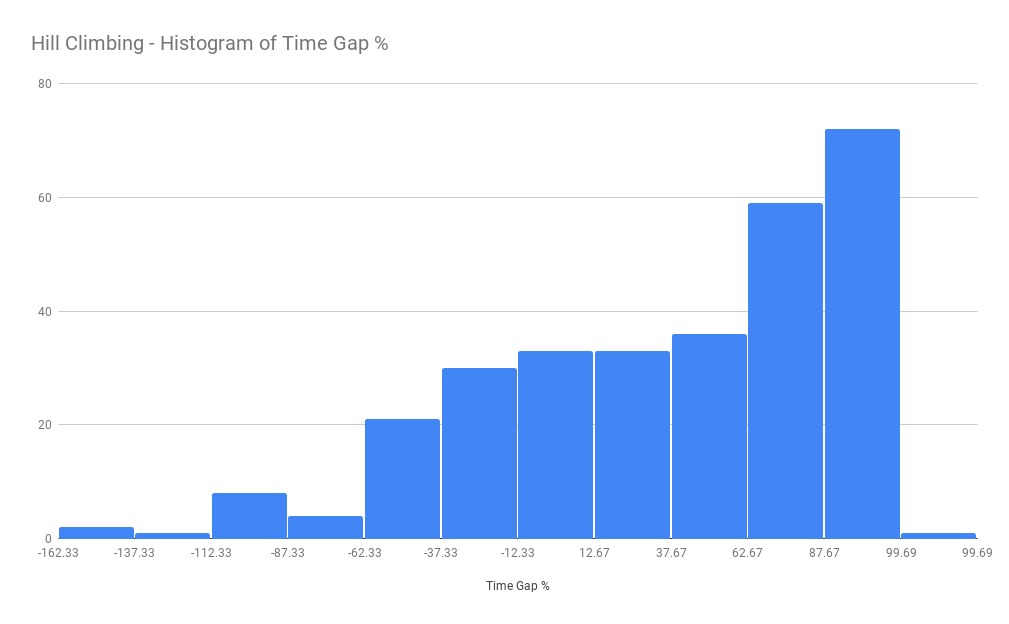
\includegraphics[width=\textwidth]{Figures/Metaheuristics/hill_climb_time_gap.png}
    \caption{LNS (Hill Climbing) Time Gap \% - positive gap means the metaheuristic method was faster}
    \label{fig:time_gap_perc_hill_climb}
\end{figure}

\begin{figure}[!htbp]
    \centering
    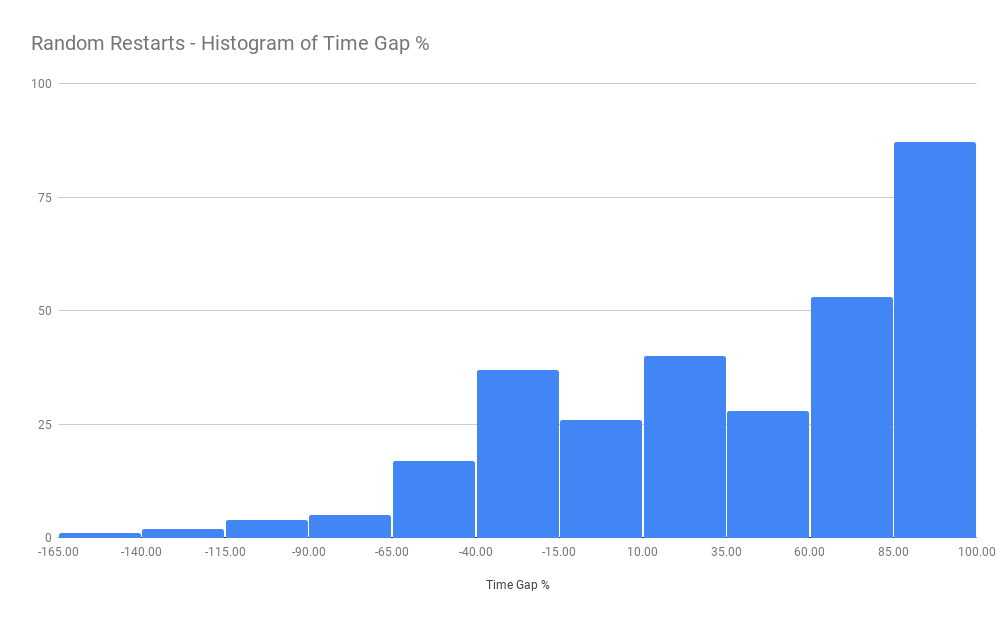
\includegraphics[width=\textwidth]{Figures/Metaheuristics/restarts_time_gap.png}
    \caption{LNS + Random Restarts Time Gap \% - positive gap means the metaheuristic method was faster}
    \label{fig:time_gap_perc_restarts}
\end{figure}

\begin{figure}[!htbp]
    \centering
    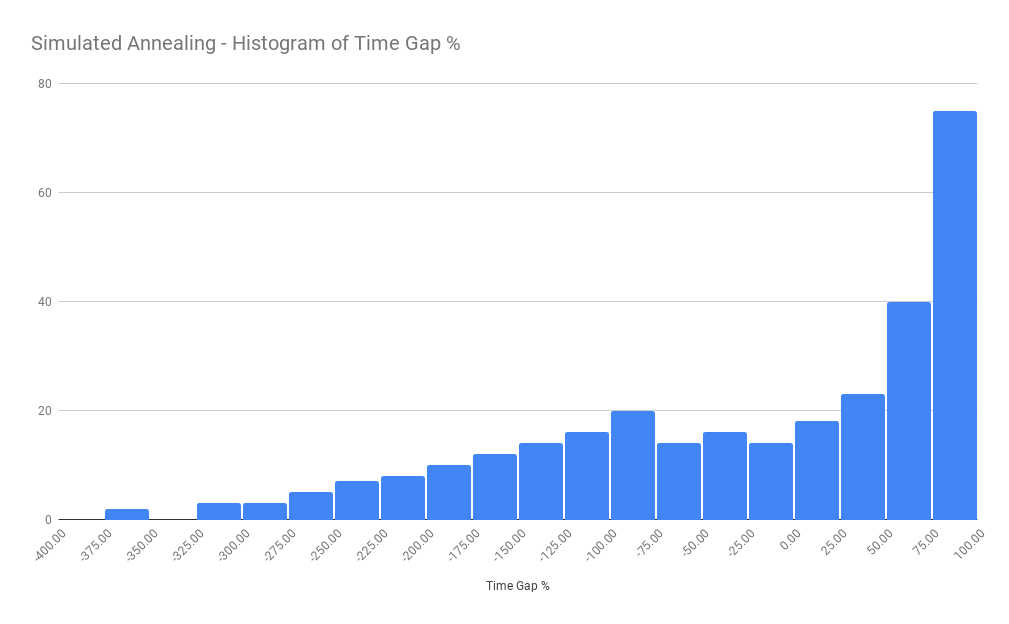
\includegraphics[width=\textwidth]{Figures/Metaheuristics/annealing_time_gap.png}
    \caption{LNS + Random Restarts + SA Time Gap \% - positive gap means the metaheuristic method was faster}
    \label{fig:time_gap_perc_annealing}
\end{figure}

\begin{figure}[!htbp]
    \centering
    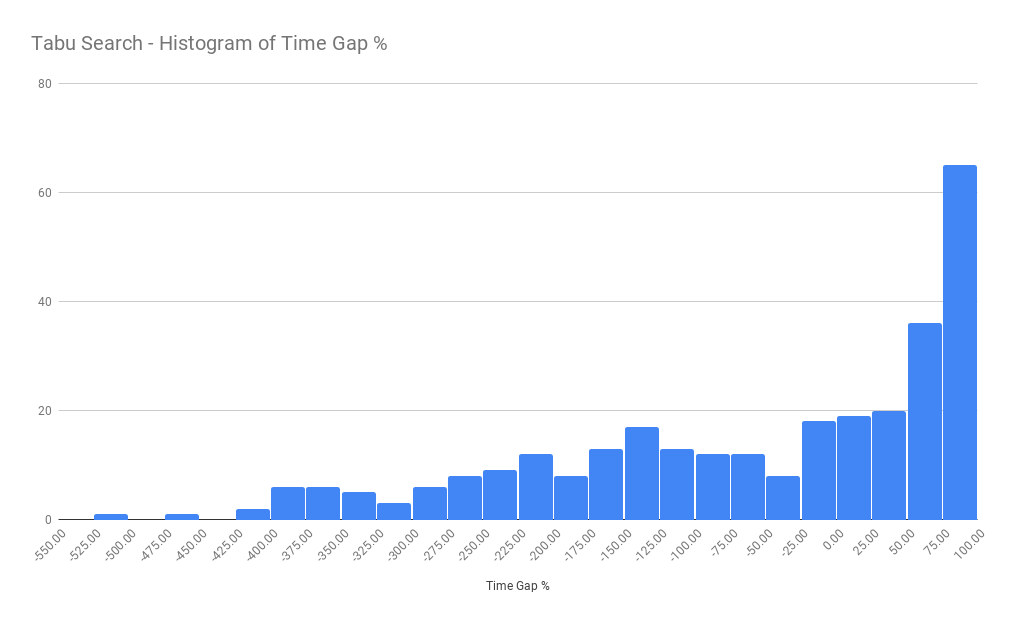
\includegraphics[width=\textwidth]{Figures/Metaheuristics/tabu_time_gap.png}
    \caption{LNS + Random Restarts + SA + TS Time Gap \% - positive gap means the metaheuristic method was faster}
    \label{fig:time_gap_perc_tabu}
\end{figure}

\FloatBarrier

\subsection{Value and Time Gaps}

Even though the search can be seen to perform well overall, it is also important to understand how and why this metaheuristic approach struggles and why the outliers occur. Take note that all figures shown in this subsection are using the combination of LNS (hill climbing), random restarts and simulated annealing since this gave the best results, and they do not include tabu search. As a reminder, the value gap represents how close the solutions produced by the metaheuristic are, where 0\% means that they are equal (the metaheuristic found the optimal) and 10\% means that the metaheuristic was 10\% below the optimal value. For the time gap, 0\% means that the metaheuristic took exactly the same time as the optimal approach, +10\% means that the metaheuristic was 10\% faster than the optimal approach, and -10\% means that the metaheuristic was 10\% slower than the optimal approach.

\Cref{fig:value_gap_vs_size} shows that the value gap is much smaller or finds the optimal solution in small problems and increases in larger problems (fluctuating around 0.74\% in these results). However, it's clear from the time gap in \cref{fig:time_gap_vs_size} that the local search is usually slower than the complete algorithm in small problems but is faster in large problems. Naturally, if the solution space is small, Branch and Bound can traverse most of it in a very short time whereas a local search with a fixed number of iterations may 'waste' some time in these cases.

\begin{figure}[h!]
    \centering
    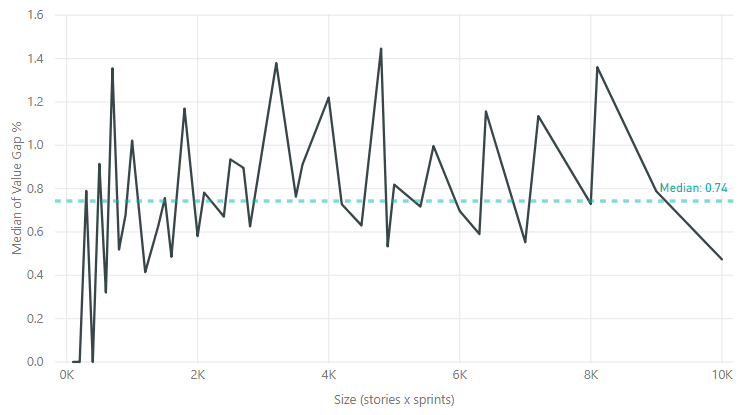
\includegraphics[width=\textwidth]{Figures/Results/annealing_value_gap_size.png}
    \caption{Value Gap \% vs Size}
    \label{fig:value_gap_vs_size}
\end{figure}

\begin{figure}[h!]
    \centering
    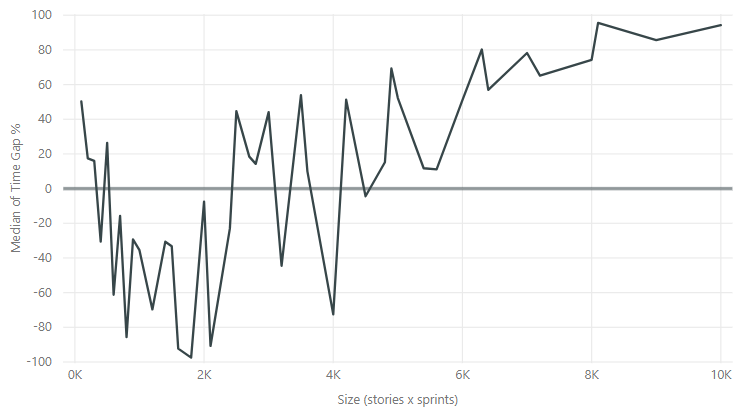
\includegraphics[width=\textwidth]{Figures/Results/annealing_time_gap_size.png}
    \caption{Time Gap \% vs Size}
    \label{fig:time_gap_vs_size}
\end{figure}

For the ratio of dependencies to stories, \cref{fig:value_gap_vs_dependencies_stories} shows that the value gap peaks between 1 and 1.2 where there are roughly the same number of stories and dependencies. This makes sense because problems that have many dependency constraints are difficult to destroy and repair effectively using greedy heuristics as there are fewer feasible ways to insert stories. The time gap in \cref{fig:time_gap_vs_dependencies_stories} shows that the local search is much faster than the optimal search around the 1 to 1.2 range. This could be because the local search is able to find a good, but not necessarily the best, neighbour at each iteration and it is able to continue searching without 'stalling' and can terminate quickly. If the optimal algorithm must find the best set of assignments to make at each iteration, it must spend more time evaluating each step. In other words, when the ratio of dependencies to stories is around 1:1, the local search is able to terminate faster than branch and bound but the value gap increases.

\begin{figure}[h!]
    \centering
    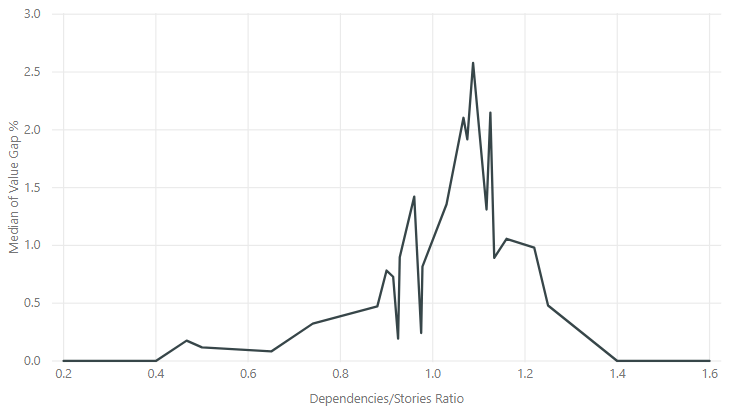
\includegraphics[width=\textwidth]{Figures/Results/annealing_value_gap_dependencies_stories.png}
    \caption{Value Gap \% vs Dependencies/Stories Ratio}
    \label{fig:value_gap_vs_dependencies_stories}
\end{figure}

\begin{figure}[h!]
    \centering
    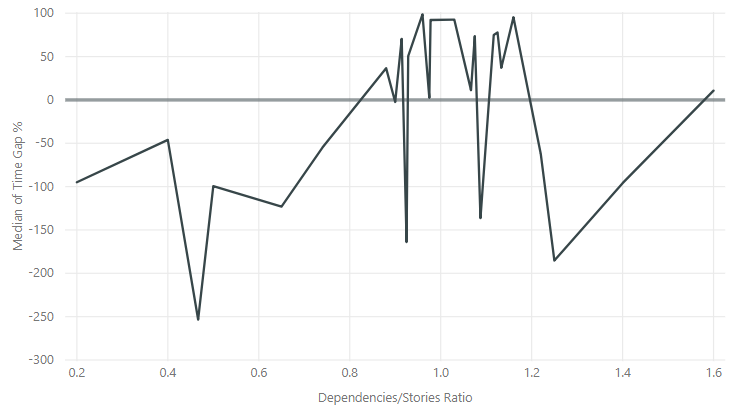
\includegraphics[width=\textwidth]{Figures/Results/annealing_time_gap_dependencies_stories.png}
    \caption{Time Gap \% vs Dependencies/Stories Ratio}
    \label{fig:time_gap_vs_dependencies_stories}
\end{figure}

For the ratio of stories to sprints, \cref{fig:value_gap_vs_stories_sprints} shows that the value gap increases as the ratio increases. This seems to be the largest explanation for the worst solutions found in all of the problems tested in this paper with the median value gap peaking around 8\%. This suggests that this local search is better at solving road maps with a longer time horizon compared to planning many stories into only a few sprints. The time gap shows that the local search generally is slower than the optimal algorithm where the ratio is low and faster it is high. As with the dependencies/stories ratio, this could be because the local search is able to spend less time at each iteration and terminate faster but in the end returns a lower-value solution than in problems where the stories/sprints ratio is low.

\begin{figure}[h!]
    \centering
    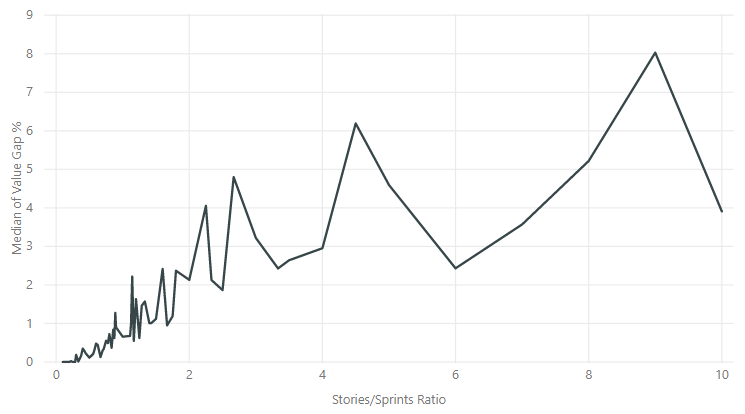
\includegraphics[width=\textwidth]{Figures/Results/annealing_value_gap_stories_sprints.png}
    \caption{Value Gap \% vs Stories/Sprints Ratio}
    \label{fig:value_gap_vs_stories_sprints}
\end{figure}

\begin{figure}[h!]
    \centering
    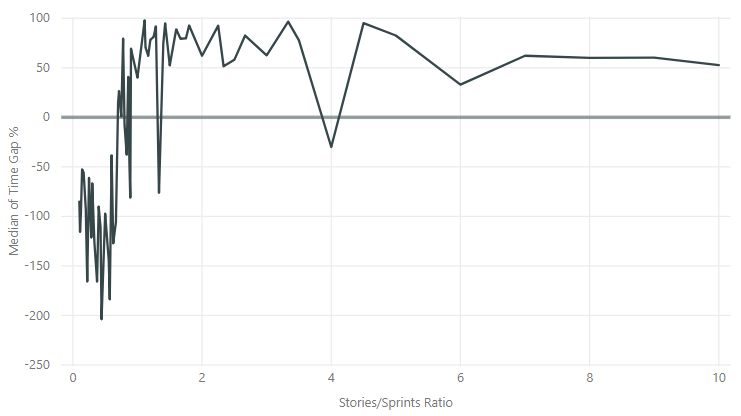
\includegraphics[width=\textwidth]{Figures/Results/annealing_time_gap_stories_sprints.png}
    \caption{Time Gap \% vs Stories/Sprints Ratio}
    \label{fig:time_gap_vs_stories_sprints}
\end{figure}
% Chapter Template

\chapter{Conclusion}
\label{ChapterConclusion}

An implementation of the ASPP was given an integer programming formulation and it was shown that it can find the optimal solution using a complete algorithm. Using warm starts was also shown to improve the time taken to find the optimal solution. The same problem was then modelled in a way that could be solved by a local search algorithm. Several popular metaheuristics such as iterated local search, simulated annealing, and tabu search were blended together to maximise the quality of solutions found by the local search. The results showed that it could find solutions that were optimal or close to optimal, depending on the size and complexity of the problem. The time taken by the local search was of orders of magnitude faster than the complete algorithm. Therefore, it can be concluded that this combination of local search metaheuristics can successfully be applied to the ASPP to provide an fast way for an agile team to plan effectively while also increasing transparency to their stakeholders about the long-term plan of their project.

The contribution of this work over existing work was the approach taken to destroy and repair a solution by focusing on using the natural structure of the dependency graph to remove related assignments during the local search. It shows that while related works have used other approaches such as particle swarm optimisation or genetic algorithms, a combination of iterated local search, simulated annealing and tabu search can give good results.

A final reflection on this thesis (and related work) is that solving the ASPP in this way treats it somewhat like it is a deterministic problem. In reality, agile frameworks are often used in projects precisely because the journey to deliver software is far from deterministic and inherently has many unexpected events and lack of precision in estimates. It may be tempting to think that formalising the problem and methodically solving it can make agile project management less of an art and more of a science, but this was not the aim of this work. It should be viewed as an effort to minimise the operational risks of mismanaging a large software development project so that an agile team can maximise its effectiveness with the estimates it has at any particular time.
\chapter{Future Work}
\label{ChapterFutureWork}

This chapter will summarise potential extensions that could be implemented in future projects to improve the effectiveness and efficiency of the work. It will discuss both the modelling of the problem and the implementation of the local search metaheuristic.

\section{Model} \label{sec:future_work_problem_modelling}

\subsection{Developer Competencies}
In the ideal agile development team, developers have the complete set of skills required to deliver any story in the backlog, and so any set of stories can be assigned to the team's sprint backlog. In reality, many teams are compromised of developers with different competencies. Therefore, simply assigning the highest-value stories to the sprint backlog is not always realistic. To illustrate this, if a team consisted of a front-end developer and a back-end developer, and the user stories relating to the front-end development have been prioritised as high value by the Product Owner, then the optimal sprint plan is to assign only front-end tasks. Clearly, this might deliver the most business value but it is not an efficient way to utilise the development team. An alternative model could be rather than assigning tasks to the team backlog, each development team member has their own personal sprint backlog which is to be optimised. The team's sprint backlog is then simply the union of each team member's personal sprint backlog.

\subsection{Additional User Story Variables}
The model in this thesis covers only the core inputs needed to create a road map. Variables like those included in \citet{golfarelli2012sprint} such as uncertainty, affinity, criticality may create the same risk of non-delivery as mishandling dependencies or sprint capacities. As \citet{wake_2003} notes, the size of a story is a function of how well it is understood, and so the uncertainty of a story can impact the reliability of its estimation. Affinity could create more coherent plans so that stories that are naturally related are worked on in the same or nearby sprints. Affinity could also be modelled as a relationship between stories and developers since it makes sense that the developers work on tasks that are similar to ones they have previously worked on. 

Additional variables could also be interesting to model. If a purely technical user story will not deliver much business value itself but will enable delivery of more business-valuable stories, 'IT Value' could give a way for the development team to prioritise these IT tasks. In many industries, there may be regulatory requirements that do not deliver much customer or IT value but still require significant development time, and a 'Regulatory Value' variable could account for this.

\subsection{Fixed Assignments}
While agile planning encourages great flexibility in the order that stories are worked on, sometimes a story (or set of stories) must be delivered on or before a certain date. If a legal or regulatory requirement has a hard deadline, the development team must deliver the required functionality on time. These tasks must therefore dominate the placement of other stories even if they have lower business value. An additional set of constraints could be added to the model to accommodate for fixing the placement of stories on or before certain sprints.

\subsection{Scaled Agile}
The focus of this thesis has been on a single agile team but the real difficulty in dependency management and creating realistic plans comes when multiple teams are working together. This not only increases the size of the problem but also the complexity when teams have dependencies in each other's backlogs. The Scaled Agile Framework (SAFe) for Lean Enterprises \citep{scaled_agile_inc_2018} offers a framework for orchestrating multiple scrum teams who are producing software towards common, high-level objectives. Program Increment Planning is a significant event were the teams essentially perform their sprint planning events all together and plan for the next 4 or 5 sprints. It requires careful planning and coordination between the teams to ensure that dependencies and risks are managed and realistic Program Increment objectives can be committed to. An algorithm that can automatically create a good plan could dramatically increase the efficiency of these events by removing the need to do manual scheduling across many scrum teams. The model would need to be extended to include the concepts associated with SAFe such as PI Objectives, Strategic Themes, Solution Trains, Portfolios, and new stakeholders such as Release Train Engineers, Solution Managers, and Enterprise Architects. Prioritisation of the high- level objectives could flow down and influence the planning decisions of the individual scrum teams to ensure that a road map not only creates value to one team but collectively adds value to the whole portfolio in an optimal way.

\section{Adaptive Metaheuristics}

A possible bottleneck of the local search's implementation is that many of the metaheuristic parameters are chosen a priori. While much effort was put into experimentally finding good parameters for the given sets of test data, it is very difficult to choose values that work well for all problems. Therefore, implementing adaptive metaheuristics that can adjust their parameters on the fly during the search may further reduce the gap in value between the local search and the optimal search results.

\subsection{Tabu Search}
The tenure of moves and size of the tabu list have a significant impact on the effectiveness of tabu search. More robust variations of tabu search suggest randomly adjusting the tenure and size rather than fixing them beforehand, but parameters such as how much variation there should be in the random values must still be chosen. Reactive Tabu Search \citep{battiti1994reactive} designs the tabu list so that the size of the list is learned automatically during the search. It tracks how often each move occurs and if moves are being frequently repeated, the size of the list is increased. When regions of the search space that do not need such a large list are being explored, the list size is slowly reduced.

\subsection{Solution Destruction}

\subsubsection{Adaptive Level of Destruction}
Deciding how much of the solution to remove can be hard. On one hand, the search could remove all related assignments (as briefly discussed in \cref{destroy}) but this eliminates the control over how much of the solution is destroyed. On the other hand, the search could remove a certain number of assignments but the exact number can change during the course of the search rather than being fixed beforehand. The general idea could be that when exploration is needed (for example to break out of a local optimum), the number of stories removed is increased to generate neighbours that are 'further away' from the current solution. Conversely, if higher-value solutions are being discovered, the search can reduce the number of stories removed to focus on intensification and polishing the current solution.

\subsubsection{Adaptive Destruction and Repair Methods}
Two ways of destroying a solution were used in this work: random and radial. These were applied alternately to give some variety in how the search generated neighbours. However, one of these methods may be more effective in progressing the search forward in different problems or in different stages of the search. It could therefore be interesting if the search tracks how well each destroy or repair heuristic performs. Intuitively, heuristics that lead the search to high quality solutions should be used more often. \citet{ropke2006adaptive} proposes a variation of Large Neighbourhood Search named \emph{Adaptive Large Neighbourhood Search} that uses a number of competing sub-heuristics which are used with a frequency corresponding to their historical performance. The idea is to keep track of a score for each heuristic and its score is increased if the last destroy-repair operation either: (1) finds a new global optimum (this is of course desirable), (2) discovers an unvisited solution that improves the current solution (it was able to find a better neighbour which had not been seen before), or (3) discovers an unvisited solution that does not improve the current solution (it was able to diversify the search to a new area, even if it didn't improve the current/global solution). This dynamic approach allows the search to favour good heuristics but also allows it to 'change its mind' about which it uses during the search as the scores are adjusted.

\subsection{Solution Repair}
Using a greedy heuristic to insert stories into a partial solution may be fast but it doesn't guarantee to create the best solution possible after repair. If the number of assignments removed is relatively small, a complete algorithm could be used as the mechanism to repair. This could reduce the amount of time spent exploring lower value solutions that are only visited because the greedy heuristic was not able to construct the best solution for a given partial solution.

\section{Code Improvements}

\subsection{Parallelism}
Local search is inherently iterative - the next iteration depends on the result on the previous one. However, parts of the code have the potential to be run in parallel to increase the amount of CPU time that the search uses to find the global optimum while possibly using less wall time.

As the size of the problem grows, the number of assignments that the constraint checking and objective function must examine grows. This can have a major influence on the overall execution time of the local search. However, simply checking the set of assignments does not require any kind of mutation so there would potentially be no race conditions if multiple threads read the assignments at the same time. In other words, the search does not need to wait for one story/sprint to have its constraints checked before processing the next. A potentially significant time boost could be gained by spawning a thread that checks the constraints for a single story/sprint (or a subset of stories/sprints) so that all are checked in parallel. Similarly, the objective function could sum the business value of each sprint in parallel and then sum the subtotals into a grand total when the threads are joined. When Tabu search is used, the local search must check every move against the tabu list. Again, reading the tabu list does not mutate it and so the code could check all moves in parallel at the same time.

Random restarts try to cover as much of the search space as possible by starting at different random positions and performing a local search. The best solution found over the multiple restarts is then returned as the final result. Instead of waiting for the first search to stagnate before starting the next one, several local searches could be spawned to traverse random parts of the search space at the same time. This draws parallels with Particle Swarm Optimisation but each thread does not necessarily need to interact with the others. Instead, a number of threads can be spawned that each runs the local search. When the threads are joined at the end, the best of the best results is returned.

\section{End-to-end Tool}
In the Model-View-Controller architectural design pattern \citep{pope1988cookbook}, applications are divided into 3 parts. The Model manages the data representation of the system, the View displays representations of the data to the user, and the Controller contains the 'business logic' that updates the view and the model. Looking at this thesis using the MVC pattern, the focus has mostly been on developing the controller. The usability of the work is minimal as little attention was paid to how the data is stored or how an agile team would view the data and interact with the results produced by the code.

\subsection{Model}
The 'static' data is stored as flat CSV files that are read in by the program. Where possible, efficient data structures are used to access the data needed by the local search - for example, stories and sprints are given an ID number and are placed in an array at the corresponding index so that they can be accessed in constant time if the ID is known. Also the tabu list is implemented using maps to allow fast look-ups of moves. However as mentioned in previous sections, the stories and dependency links can be seen as a directed, acyclic graph where nodes are stories and edges are dependency links. This model fits naturally with the concepts of a graph database and operations that must traverse the graph may benefit from representing the data in this way compared to the flat structure used in this project. Additionally, the extensions to the modelling of the problem covered in \cref{sec:future_work_problem_modelling} also fit with a graph database if one uses different types of nodes to represent developers, skills etc that are connected by edges representing the relationships between them.

While storing the static data of the problem in a graph database may have its advantages in terms of looking up the constant values associated with stories and sprints, it could also be an interesting way to represent a solution in the local search. If one type of node represents a sprint and another represents a story, a directed edge from a story to a sprint could represent that the story is assigned to the sprint. The code to destroy a solution could be greatly simplified by replacing a C++ implementation of breadth-first search with a simple graph database query. As well as simplifying the code, it would decouple the 'business logic' from the model of the data by no longer requiring that the controller must know how to traverse the relationships between the static data in the model. The process of destroying and repairing a solution could therefore be to disconnect and reconnect stories from sprints in the graph database.

Furthermore, a hybrid of these two points may be an even more intuitive and powerful way to model the problem where stories are connected to sprints by an 'assigned to' edge, and stories are connected to each other by 'depends on' edges. The local search algorithm could then have a single model where it can look up static data, generate neighbours, and check the constraints.

An extension that goes hand in hand with using a database could be to implement some integration with popular commercial agile project management tools like JIRA so that a team can simply import their existing backlog into the model ready to be solved.

\subsection{View}
Since the test data was generated automatically, building a user-friendly way to create and interact with the backlog was low priority. If the implementation is to be used by a real agile team, some kind of user interface would be necessary so that they are able to view and edit the stories (and dependencies) and sprints. If a database is used to persist the data, this user interface could just be a standard rows and columns view that allows the user to edit the static data. The interface could also be a custom visualisation of the graph structure of the model which may be a more intuitive way to work with it.

%----------------------------------------------------------------------------------------
%	THESIS CONTENT - APPENDICES
%----------------------------------------------------------------------------------------

\appendix % Cue to tell LaTeX that the following "chapters" are Appendices

% Include the appendices of the thesis as separate files from the Appendices folder
% Uncomment the lines as you write the Appendices

%% Appendix A

\chapter{Frequently Asked Questions} % Main appendix title

\label{AppendixA} % For referencing this appendix elsewhere, use \ref{AppendixA}

\section{How do I change the colors of links?}

The color of links can be changed to your liking using:

{\small\verb!\hypersetup{urlcolor=red}!}, or

{\small\verb!\hypersetup{citecolor=green}!}, or

{\small\verb!\hypersetup{allcolor=blue}!}.

\noindent If you want to completely hide the links, you can use:

{\small\verb!\hypersetup{allcolors=.}!}, or even better: 

{\small\verb!\hypersetup{hidelinks}!}.

\noindent If you want to have obvious links in the PDF but not the printed text, use:

{\small\verb!\hypersetup{colorlinks=false}!}.

%\include{Appendices/AppendixB}
%\include{Appendices/AppendixC}

%----------------------------------------------------------------------------------------
%	BIBLIOGRAPHY
%----------------------------------------------------------------------------------------

\printbibliography[heading=bibintoc]

%----------------------------------------------------------------------------------------

\end{document}  
